%!TEX encoding = UTF-8 Unicode
\documentclass[11pt,a4paper,papersize,oneside]{jsbook}

\usepackage[OT2,T1]{fontenc}
\usepackage{amsmath}
\usepackage{amssymb}
\usepackage{newtxtext,newtxmath}
\usepackage[dvipdfmx]{graphicx}
\graphicspath{{Fig/}}
\usepackage{url}
\usepackage[dvipdfmx]{hyperref}
\usepackage[dvipdfmx]{pxjahyper} % 日本語のhyperref
\usepackage{makeidx}\makeindex  % allows for indexgeneration

\usepackage{pifont}
\usepackage{array,booktabs}
\usepackage{setspace}
\usepackage{enumitem}

% PDF meta information and bookmarks
\hypersetup{
bookmarks=true,         % show bookmarks bar?
bookmarksnumbered=true,
bookmarkstype=toc,
%unicode=true,          % non-Latin characters in Acrobat’s bookmarks
pdftoolbar=true,        % show Acrobat’s toolbar?
pdfmenubar=true,        % show Acrobat’s menu?
pdffitwindow=false,     % window fit to page when opened
pdftitle={推薦システムのアルゴリズム},    % title
pdfauthor={神嶌 敏弘},     % author
pdfsubject={}, % subject
pdfkeywords={推薦システム;recommender system;協調フィルタリング;collaborative filtering}, % list of keywords
pdfnewwindow=true,      % links in new window
%setpagesize=false, % setting paper size
}

% local macro definitions
\usepackage{mathsymbols}
\usepackage{myindex}

% set pagesize: A4paper, margin=3cm
\setlength{\topmargin}{4.6truemm}
\setlength{\headheight}{1\baselineskip}
\setlength{\headsep}{1\baselineskip}
\setlength{\textheight}{\paperheight}\addtolength{\textheight}{-60truemm}\addtolength{\textheight}{-2\baselineskip}
\setlength{\footskip}{0pt}
\setlength{\oddsidemargin}{4.6truemm}
\setlength{\evensidemargin}{\oddsidemargin}
\setlength{\textwidth}{\paperwidth}\addtolength{\textwidth}{-60truemm}
\setlength{\fullwidth}{\textwidth}

%%%% more linebreaks in equations %%%%

\binoppenalty=0
\relpenalty=0
% \mathcode`\,="202C      % "," is considered as a binary operator

%%%%% condense floats %%%%%

%\def\topfraction{0.99}
%\def\bottomfraction{0.01}
%\def\textfraction{0.01}
%\def\floatpagefraction{0.99}
%\def\dbltopfraction{0.99}
%\def\dblfloatpagefraction{0.99}

%%%%% title, author, and release %%%%%

\title{\LARGE\textbf{推薦システムのアルゴリズム}}
\author{\textbf{神嶌 敏弘}\quad$\langle$\url{http://www.kamishima.net/}$\rangle$}
\date{Release: \input{version}}

\begin{document}

% ===== Front Matter =====
\frontmatter

% --- Title ---
\maketitle

% --- Preface & Notation---
\onehalfspacing

%!TEX root =  main.tex
%!TEX encoding = UTF-8 Unicode
\chapter*{まえがき}
\label{chap:preface}

本稿は推薦システムについてまとめたものである.

人工知能学会誌2007年11月号~\cite{jpublist:076},2008年1月号~\cite{jpublist:081},および2008年3月号~\cite{jpublist:083}の3回に渡って連載した解説記事「推薦システムのアルゴリズム(1)〜(3)」に対し,誤りの訂正や,新しい内容の追加などの更新を行ったものである.

本稿のソースファイルは \texttt{GitHub} にて公開している.
\begin{quote}
\url{https://github.com/tkamishima/recsysdoc}
\end{quote}
TYPOや記述の誤りなどのバグリポートは,\texttt{GitHub} の rull request か,issues を使って連絡されたい.
なお,事情によりすぐには対処できない場合があるので,予めご了解いただきたい.

\section*{本稿の構成}
\label{sec:preface-organization}

本稿の構成は以下のとおりである.
第\ref{part:overview}部では,推薦システムとは何か,またその設計指針や分類について述べる.
第\ref{part:process}部では,データの入力,嗜好の予測,そして推薦の提示からなる推薦システムの実行過程について述べる.
第\ref{part:algoirthm}部では,さまざまな嗜好の予測アルゴリズムのを紹介する.
第\ref{part:topic}部では,推薦システムに関連する話題や,さまざまな状況での推薦を紹介する.
第\ref{part:conclusion}部は関連資料の紹介とまとめである.

%!TEX root =  main.tex
%!TEX encoding = UTF-8 Unicode
\chapter*{数式の表記}
\label{chap:notation}

スカラーの変数はイタリック体 $x$ で,一部の確立変数は大文字のイタリック体 $X$,ベクトルは小文字ボールド体 $\bfx$で,行列は大文字ボールド体 $\bfX$で表記する.
実数などの特殊なものを除き,集合にはカリグラフィック体 $\calD$ を用いる.

\begin{center}
\small\renewcommand{\arraystretch}{0.8}
\begin{tabular}{@{}>{\centering}p{0.09\fullwidth}@{\hspace{0.01\fullwidth}}p{0.38\fullwidth}@{\hspace{0.04\fullwidth}}>{\centering}p{0.09\fullwidth}@{\hspace{0.01\fullwidth}}p{0.38\textwidth}@{}}\toprule
\textbf{表記} & \textbf{意味} & \textbf{表記} & \textbf{意味} \\ \cmidrule(r){1-2}\cmidrule{3-4}
$x$ & 特定の利用者を表す & $y$ & 特定のアイテムを表す \\
$X$ & 利用者を表す確率変数 & $Y$ & アイテムを表す確率変数 \\
$\bfx$ & 利用者をまとめたベクトル & $\bfy$ & アイテムをまとめたベクトル \\
$n$ & 利用者数 & $m$ & アイテム数 \\
$\calX$ & 利用者集合 $\{1,\ldots,n\}$ & $\calY$ & アイテム集合 $\{1,\ldots,m\}$ \\
$\calX_y$ & アイテム$y$を評価した利用者の集合 & $\calY_x$ & 利用者xが評価したアイテムの集合 \\
$a$ & 活動利用者を表す & $r_{xy}$ & 利用者$x$のアイテム$y$への評価値 \\
$\bar{r}_x$ & 利用者$x$による評価値の平均 & $\tilde{r}_y$ & アイテム$y$への評価値の平均 \\
$\bfR$ & 評価値行列 & $\calR$ & 評価値集合(5段階評価なら $\{1,\ldots,5\}$) \\
$\bfr$ & 評価値をまとめたベクトル & $z$ & 潜在因子 \\
$\bfz$ & 潜在因子のベクトル & $K$ & 潜在因子の数・次元数 \\
$\calD$ & データ集合 & $N$ & 訓練データ数 \\
$\bfU$ & 利用者潜在因子行列 & $\bfV$ & アイテム潜在因子行列 \\
$\bfu_{x}$ & 利用者$x$の潜在因子ベクトル & $\bfv_{y}$ & アイテム$y$の潜在因子ベクトル \\
$y^{(t)}$ & 時刻$t$での値 & $\ang{Y^{(t)}}$ & アイテムの時系列 \\
$\theta\,\bftheta\,\bfTheta$ & パラメータを一般に表す & $\sig()$ & シグモイド関数 \\
$\Dom()$ & 変数の定義域 & $\nan$ & 欠損値 \\
\bottomrule
\end{tabular}
\end{center}

スカラー関数 $f(x)$ に対して,その引数をベクトルとする表記 $f(\bfx)$ は,ベクトル $\bfx$ の各要素を関数 $f$ に適用して得られるベクトルを表す.

確率変数 $X$ が離散の場合の確率質量関数も,連続値の場合の確率密度関数も特に区別することなく $\pb{X}$ と表記する.

$\expect_{\pb[X]}[f(X)]$ は,分布 $\pb{X}$ についての次の期待値を表す:
\[
\begin{array}{l@{\text{ \makebox[3zw]{\dotfill} }}l}
\sum_{x\in\Dom(X)} f(x) \pb{X=x} & \text{$X$が離散の場合}\\
\int_{x\in\Dom(X)}  f(x) \pb{X=x} dx & \text{$X$が連続の場合}
\end{array}
\]
なお,$\pb{X}$を省略した場合は,関数$f$の全ての確率変数の同時分布に関する期待値を表す.例えば,$\expect[f(X,Y)]$ は,$\expect_{\pb{X,Y}}[f(X,Y)]$ の意味である.


% --- Table of Contents ---
\tableofcontents

% ===== Main Matter =====
\mainmatter

% ---- Main Content ----

\part{推薦システムの概要}
\label{part:overview}
%!TEX root =  main.tex
%!TEX encoding = UTF-8 Unicode
\chapter{推薦システム}
\label{chap:intro}

「\term{推薦システム}{recommender system}」とは,利用者にとって有用と思われる対象,情報,または商品などを選び出し,それらを利用者の目的に合わせた形で提示するシステムである.

最初に,この推薦システムが必要になった背景について述べよう.
第一に,大量の情報が発信されるようになったことがある.
これは,情報化技術の進展により,個人・団体が容易かつ低コストで発信できるようになったためである.
第二の理由は,これら大量の情報の蓄積や流通が容易になり,誰もが大量の情報を得ることができるようになったことである.
これも計算機の記憶媒体の大規模化や,通信の高速化によるものである.
以上のことから,大量に発信された情報を,だれもが大量に取得できる状況が生じた.
しかし,欲しい情報が何か分からない(例:統計資料として公開されているがその名前が分からない)とか,探している情報を見つけ出せない(例:類似した資料が大量にあり目的のものが埋もれてしまう)といった理由により,情報を参照できる状態にあるにもかかわらず,それを利用できないという状況が生じた.
この状況を「\term{情報過多}{information overload}~\cite{misc:009}
\footnote{情報爆発 (information explosion) や情報洪水 (information overflow) ともいう.}
という.
この状況を打破するため,利用者にとって有用な情報を見つけ出す推薦システムが考案された.

この推薦システムは,広い立場からみれば,情報検索や情報フィルタリング技術の一つと見なせる.そのため,初期の推薦システムは,これらの技術が基盤となっていた.
\ref{chap:process}章で述べるように,このシステムの実現手法には協調フィルタリングと内容ベースフィルタリングがある.
だが,協調フィルタリングという語の方が推薦システムより古く,1992年に文献 \cite{macm:92:01} にて使われた.
だが,これは現在のような協調フィルタリングではなく,他人が手動で行った推薦を検索できる協調作業支援のシステムであった.
この過程を自動化した協調フィルタリングが1994年のGroupLens\cite{cscw:94:01}やRingo \cite{sigchi:95:02}であり,現在の推薦システムの基礎となった.
一方の内容ベースフィルタリングの技術は,従来からある情報フィルタリングとみなせ,また,事例ベース推論の応用としても研究されてきた.
そのうち,推薦システムとして独自の側面が強くなり,協調フィルタリングに対して内容ベースフィルタリングと呼ばれるようになった.
1996年には,専門のワークショップも開催されるほどに研究が活発化した.
1997年にはACM Communications誌で特集\cite{macm:97:01} が掲載され,この種のシステムの呼び名として「Recommender System」が定着した.
このころから,NetPerceptions や Firefly などの企業によってシステムの商業化が始まった.
現在では,Webを通じた各種サービスの機能で活用されたり\cite{ieeem:99:02,ieeem:03:01,www:07:01},セットトップボックスなど
の機器に組み込まれたり\cite{kdd:04:11}している.
その後,物理的な店舗面積に商品数が制限されない電子商取引の発展や,大量の画一的な商品から,少量多品種への消費傾向の変化にに伴って,その重要性も広く認識されるようになった.
それを象徴する Amazon.com CEOのJeff Bezosの発言を引用しておこう\cite{dmkd:01:01}%
\footnote{J.~Riedlのメールによれば,J.~Bezosは,この発言を幾つかの講演で行った.ここでは,300万人と書いたが,そのときどきの顧客数に応じて,この数字は変えて用いられた.} .
\begin{center}
\cornersize*{2zw}\setlength{\fboxsep}{1zw}
\ovalbox{\begin{minipage}{0.92\linewidth}
\large\itshape
If I have 3 million customers on the Web,\\
\hfill{}I should have 3 million stores on the Web

\small\rmfamily\centering
(Webに3百万人の顧客がいるなら,3百万のWebストアを用意すべきだ)
\end{minipage}}
\end{center}
現在では,推薦システムは多方面で利用され,研究も継続的に行われ,多様な方法が目的に応じて考案されている.
これらの推薦システムの設計指針やアルゴリズムについてまとめる.

%!TEX root =  main.tex
%!TEX encoding = UTF-8 Unicode
\chapter{推薦システムの分類と目的}
\label{sec:rsysgoal}

本節では,推薦の個人化の度合いの分類と,運用側と利用者側のそれぞれ目的によるシステムの分類について述べる.
これらの目的を考慮して,推薦システムの設計方針を決めることになる.

その前に,推薦システムに関連する技術と,それらとの違いについて述べておく.
まず,情報検索における情報フィルタリングがある.これは,逐次的に入力される情報から,利用者の関心や興味を記述した利用者プロファイルに適合するものを選別する技術\cite{jb:012:00}で,推薦システムと良く似ている.
だが,主にテキスト文書を扱い,利用者プロファイルも主に索引語で示す点や,必要なものを取り出すより,不要なものを除外することが主目的である点などがが異なる.
他に,マーケティングの技術とも関連がある.
しかし,マーケティングが供給側の視点に立つのに対し,推薦システムは消費側である.推薦システムの推薦が利用者に受け入れられるためには,推薦が実際に客観的なものであり,また,そのことを利用者に示す工夫が必要になる.
また,マーケティングでは,レポートなど全体の傾向などを分析して報告することが必要だが,推薦システムにはそうしたことは要求されない.
また,マーケティングでは,顧客を客層に分類し,それに応じた対処を行うが,推薦システムでは,利用者のグループ化は目的ではない.

\section{推薦の個人化の度合い}
\label{sec:plevel}

最初に,推薦の個人化の度合いの3段階\cite{dmkd:01:01}を示す.

\begin{figure}
\centering
\begin{minipage}{0.45\fullwidth}
\centering
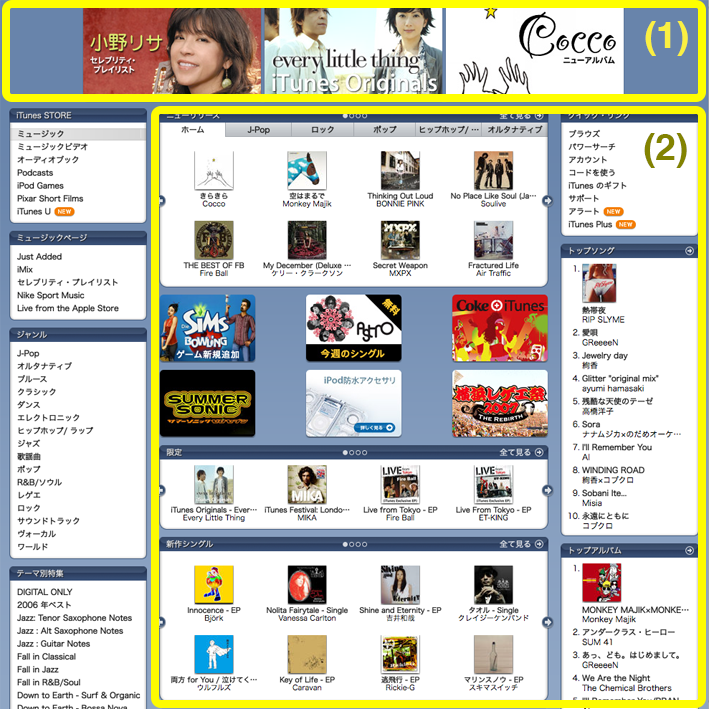
\includegraphics[width=\textwidth]{example1.png}\\
(a)~非個人化 (iTunes Store)
\end{minipage}
\hspace{0.02\fullwidth}
\begin{minipage}{0.45\fullwidth}
\centering
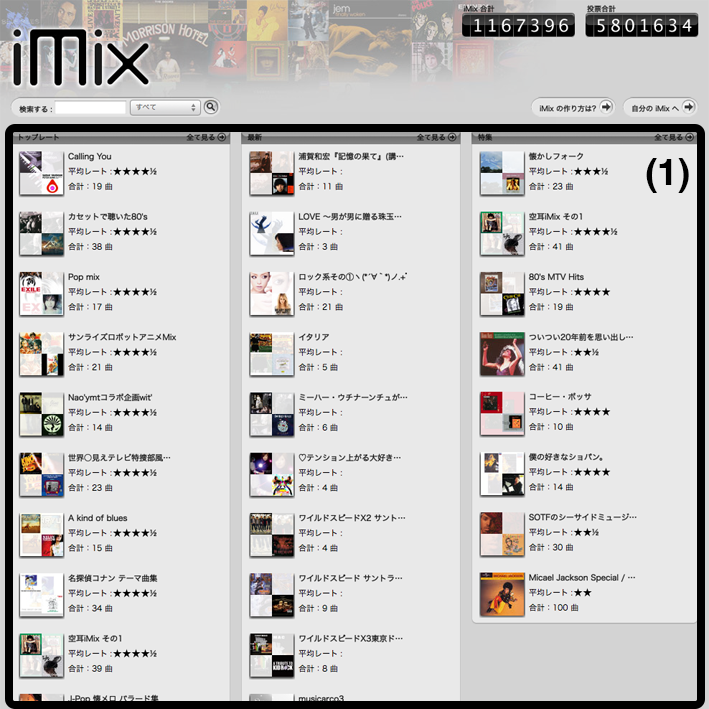
\includegraphics[width=\textwidth]{example2.png}\\
(b)~非個人化 (iTunes Store)
\end{minipage}
\medskip\\
\begin{minipage}[b]{0.45\fullwidth}
\centering
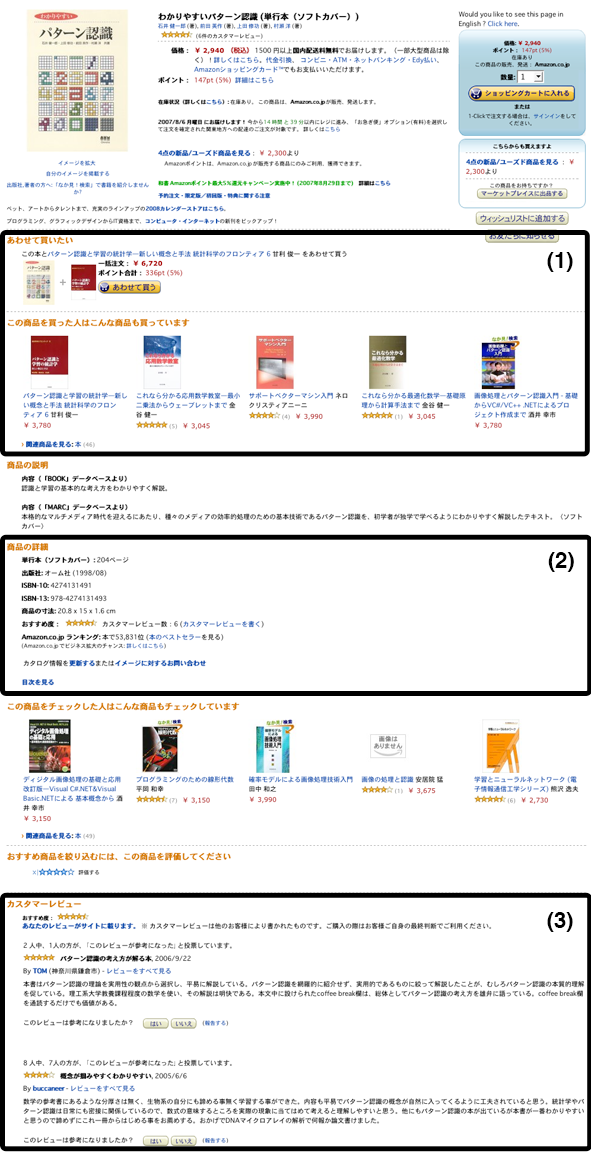
\includegraphics[width=\textwidth]{example56.png}\\
(c)~一時的個人化 (Amazon.co.jp)
\end{minipage}
\hspace{0.02\fullwidth}
\begin{minipage}[b]{0.45\fullwidth}
\centering
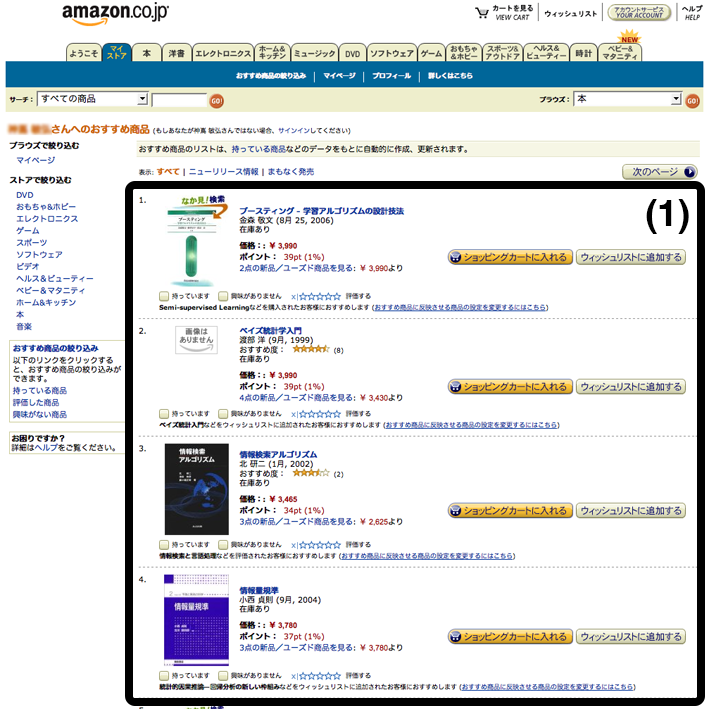
\includegraphics[width=\textwidth]{example4.png}\\
(d)~永続的個人化 (Amazon.co.jp)
\end{minipage}
\bigskip\\
\caption{個人化の度合いの異なる推薦の例}
\label{fig:plevel}
{\footnotesize 図(a),(b),(d) は2007/07/26日に,図(c)は2007/08/04日にスクリーンショットを取得した.}
\end{figure}

\begin{description}[style=nextline]
\item[\term{非個人化}{no personalization}]
全ての利用者について,全く同じ推薦をする場合である.
例えば,編集者による推薦や,売り上げ順位リストなどである.
推薦システムというときは個人化かつ自動化されたものを想定するかもしれないが,こうしたものも広義には含める.
非個人化の推薦の例を図\ref{fig:plevel}(a)と(b)に示す.
図\ref{fig:plevel}(a)中の,(1)は店舗の編集者が手作業で選んだもの,(2)は予約や売り上げの順位リストである.
システム側だけでなく,図\ref{fig:plevel}(b)のように,他の利用者が手作業で作成する推薦リストもある.
\item[\term{一時的個人化}{ephemeral personalization}]
システムを利用する一つのセッションで同じ入力や振る舞いをした利用者には,同じ推薦をする場合である.
一時的個人化の推薦の例を図\ref{fig:plevel}(c)に示す.
この例では,利用者がある本を閲覧するという行動をシステムに対してしたとき,その本に関連する情報を示している.
図中の,(1)はこの本と関連が深い本を推薦し,(2)には,書誌情報や売り上げ順位など,(3)では他の利用者の評価やコメントなど,この本についての関連情報を提示している.
\item[\term{永続的個人化}{persistent personalization}]
たとえ同じ入力や行動をシステムにしている利用者でも,利用者の個人情報や過去の利用履歴に応じて異なる推薦をする場合である.
例えば,過去の購入・利用履歴に基づいて推薦したり,年齢に応じて推薦するアイテムを変えたりする.
永続的個人化の推薦の例である図\ref{fig:plevel}(d)では,この利用者の過去の商品への評価に基づいて,関心があるであろう本を予測し,順位付けして提示している.
\end{description}

\section{推薦システムの運用目的の分類}
\label{sec:systemtarget}

次に,推薦システムを,運用側の目的に基づいて分類する.
文献\cite{dmkd:01:01}では,自動・手動の推薦システムを次の5種類に分
類し,目的に応じて適切に組み合わせて利用すべきと述べている.

\begin{description}[style=nextline]
\item[概要推薦 (broad recommendation)]
これは,全体の統計情報や運用者側の編集者を使う場合である.
全体の統計情報とは「今週の売り上げランキング」や「個々の商品の売り上げ順位」といったもので,編集者による推薦には「評論家が推薦する映画」や「特売品リスト」などがある.
図\ref{fig:plevel}(a)はこうした概要推薦の例である.
こうした概要推薦は,システムを利用し始めたばかりか,ごくまれにしか利用しないような利用者を対象とする.
これらの利用者が,自身の要求との関連性を見いだして,システムの利用を続けてもらえるように,大まかな情報を提供するのが目的である.
よって,積極的に探さなくても見えるように,システムにアクセスしたとき最初に見える場所に配置するべき推薦である.
加えて,利用者が積極的にシステムに働きかけることは期待できないので,非個人化または,アイテムのカテゴリを示す程度の入力に対応した一時的個人化した推薦をすべきである.
\item[利用者評価 (user comments and rating)]
これは,運用側が用意したシステム上で,利用者間での推薦をする場合である.
例えば,読者の批評文や★の数で示した評価レートをつけられるようにし,それらを他の利用者が参照したり,平均評価値などの統計情報を見たりできるようにする.
図\ref{fig:plevel}(b)のような他の利用者による推薦リストや,図\ref{fig:plevel}(c)の(3)のように他の利用者による評価やコメントなどが
この種の推薦の例である.\par
一般に,運用側のシステムが第三者的な立場で推薦しているとは,利用者にはあまり思われない.
それに対し,他の利用者の方がずっと信用され,その推薦も受け入れられやすい.
運用側には,システムに対する利用者の信頼を高めたり,利用頻度を高めたりといった利点がある.
こうした推薦は,運用側の関与は少なく,評価値順のアイテムリストなどの非個人化か,閲覧中のアイテムの評価値やコメントなどの単純な一時的個人化が行われる.
\item[通知サービス (notification service)]
これは,利用者がシステムを操作していないときに,電子メールなどで推薦を配送する場合である.
一つには,過去の購買履歴に基づいて,新規のアイテムの中から推薦リストを生成し,利用者に送付するといった,永続的個人化をするものがある.
また,利用者が予め設定した条件,例えば,ファンである歌手などを設定しておくと,その歌手の新譜の案内が届くという一時的個人化をした推薦もある.
これらの推薦は,システムの再利用を利用者に促すことを目的とする.
\item[関連アイテム推薦 (item-associated recommendation)]
利用者が注目している,例えば,電子商取引サイトで,商品を閲覧しているとか,「買い物かご」にすでに商品を入れている状況を想定する.
このとき,注目しているアイテムの比較候補(例:他メーカーの同等品)を示して,購入の判断を助けたり,購入の決断を促す場合や,補足的な商品などを提示してcross-selling(例:ハンバーガーにポテトなどの関連品を薦めて同時に購入させる)を促す場合がこの種の推薦である.
例としては,図\ref{fig:plevel}(c)の(1)のように閲覧中の商品の関連商品を示すものがある.
注目している商品の情報だけに基づく一時的個人化も,利用者の過去の行動も考慮する永続的個人化も可能である.
\item[緊密な個人化 (deep personalization)]
システムが積極的に利用者の情報を能動的に収集したり,過去の行動の情報を蓄積し,それらに基づいて推薦を行う場合である.
図\ref{fig:plevel}(d)のような,個人向けの推薦リストなどが,この種の推薦に該当する.
利用者がシステムを利用し続けることで蓄積された情報に基づいて,永続的な個人化が可能になる.すると,より適切な推薦ができるようになり,他のシステムとの差別化につながり,利用者の長期間にわたるロイヤリティ構築に役立つ.
だが,一方で,最も実装に困難が伴い,コストも要する.
\end{description}

\section{推薦システムの予測タスクの分類}
\label{sec:recomtask}

推薦システムが達成するタスクに基づく分類を文献\cite{jacm:04:01,jmlr:09:01}に沿って示す.

\begin{description}[style=nextline]
\item[\termmain{適合アイテム発見}{finding some good items}]
このタスクの目的は,利用者が自分の嗜好に適合するものを,何か見つけ出すことである.
利用者が積極的な動機を持って,情報を見つけるために推薦システムを利用するときは,こうした目的になる.\par
例えば,今から食べに行く店を決めるために,レストラン推薦システムを利用することが想定される.
この場合には,予測される評価の高い,比較的少数のものに絞り込んで利用者に提示する.
利用者はこのリストを上位から閲覧することで,自身の決定に必要な情報を知ることができるだろう.
\item[\termmain{評価値予測}{predicting ratings}]
このタスクの目的は利用者がアイテムに付けるであろう評価値を予測することである.
何らかのフォーマットに従ってアイテムが整列されていたり,構造化されている状況を考える.
例えば,新商品を発売日が直近になるように整列したり,カテゴリ別に商品を分類したり,メールや掲示板で記事をスレッド状に表示したりする場合である.
このように整列されたアイテムを,利用者が閲覧しているとする.このとき,閲覧の順序を決めたりとか,どの記事を閲覧するかとかを決めるために,手がかりとなる情報があれば便利である.
そのような情報として,利用者が関心をもつ度合いを,システムは予測して付随的に提示する.
適合アイテム推薦とは違って,利用者には,必ずしも,最終的に意志決定をするような積極的な動機があるとは限らず,また,関
心のあるものを特に選んで表示するといった,アイテムの提示フォーマットを変えるような要求もない.\par
例えば,決まった予定はないが,レストランの紹介Webサイトなどを閲覧しているときなどである.
レストランは,料理の種別や,推薦の度合いは,★の数や,アイコン,グラフなどを対象と共に表示す
ることで利用者に提示する.この推薦情報は,多数のレストランの中から,利用者にとって関心のあるものを絞り込むのに役立つ.
\item[\termmain{適合アイテム列挙}{finding all good items}]
このタスクの目的は,利用者が自分の嗜好に適合するものを網羅的に見つけ出すことである.
これは裏返しに,適合しないものを排除する目的であるともいえる.
例えば,会社の法務部門が関連する特許や判例を検索したり,スパムメールの可能性がないメールだけを閲覧したいといった場合である.
\item[\termmain{効用最適化}{optimizing utility}]
このタスクの目的は,何らかの効用関数を設定し,それを最適化するようなアイテムを見つけることである.
適合するアイテムなら1,それ以外は0という効用関数を考えると,適合アイテム発見はこの効用最適化とみなせるので,適合アイテム発見を一般化したタスクと考えることができる.
例えば,電子商取引サイトで推薦システムによって利益を増やす場合に,元から購入を意図していたアイテムに追加のアイテムを購入させるという組み合わせ販売 (cross-selling) \index{組み合わせ販売}\index{cross-selling}を促進するような効用関数を設定したりする.
\end{description}

\section{推薦システムの利用動機の分類}
\label{sec:usertarget}

文献\cite{sigir:01:01}では,利用者の推薦システムの利用動機の分類を示している.
前者のタイプほど,既知のアイテムに近い推薦することが望まれる.
\begin{description}
 \item[備忘録 (reminder)] 既知のアイテムを思い出させる.
 \item[類似品 (more like this)] 比較などのため既知のアイテムに類似したものを探す.
 \item[新規アイテム (new items)] 自分が確実に好むであろう,未知の新製品を探す.
 \item[視野を広げる (broden my horizon)] 他のジャンルにも自分の関心を広げる.
\end{description}

%!TEX root =  main.tex
%!TEX encoding = UTF-8 Unicode
\chapter{推薦システム設計の要素}
\label{chap:design}

多種多様な推薦システムのためのアルゴリズムが存在するが,一体,どのアルゴリズムを使えばよいのであろうか?
機械学習の基本的な定理であるノーフリーランチ定理によれば万能アルゴリズムは存在しない.
よって,アルゴリズムは,推薦システムを利用する目的や,推薦を実行する環境の制約に応じて選択する必要がある.
ここでは,そのために考慮すべき要因を大きく二つに分けて述べる.
一つは,推薦の性質である.\ref{sec:recomtask}節の利用者の目的などに応じて,推薦は適切な性質を備えるべきである.この性質を測るための規準を幾つか示す.
もう一つは,推薦を計算するためのデータや計算機資源の制約である.データや計算機資源は無限にはなく,何らかのトレードオフを考慮しつつ推薦システムは設計する必要がある.

\section{推薦の性質}
\label{sec:recomtype}

推薦システムでは,利用者が好むものを予測して提示する.
だが,利用者が何を好むかは,利用者の目的,システムを利用する状況,推薦の候補などによって変化する.
よって,提示する推薦の性質を決めるにあたって考慮すべき規準があれば役立つ.
これらの規準を以下に示す.
なお,推薦の質の評価については,文献\cite{jacm:04:01,jmlr:09:01}が詳しい.
%@@@ 推薦の質の評価の章ができたらそこへリンク
%@@@ 予測精度の評価の章を作ったら,そこに指標の説明を動かす

\subsection{予測精度}
\label{sec:prederr}
\index{予測精度}\index{accuracy}


予測精度とは,予測して推薦したアイテムに,実際にどれくらい利用者が関心をもつかという規準である.
利用者が関心のないアイテムを推薦しても役に立たないので,予測精度は最も重視すべき規準である\cite{sigir:01:01}.
評価はオンラインで行う場合と,オフラインで行う場合がある.
オンラインでの評価とは,被験者に実際にシステムを利用させ,推薦が適合したかどうかを調査するものである.
一方,事前に被験者から集めた嗜好データと,予測した結果の一致を調べるのがオフラインでの評価である.
前者の方がより実際の運用に近い評価ができるが,この調査のコストは高い.そのため,得られるデータ数が少なく安定した検証が困難であったり,多数の項目での比較が困難になるなどの問題がある.
こうした点ではオフラインでの評価の方が有利になる.

オンラインの評価では,それぞれのアルゴリズムを利用させて,推薦を利用者が受け入れる比率で,アルゴリズムの相対的な予測精度を評価する.
また,二つのアルゴリズムによる推薦リストの上位から交互にアイテムを選んで,一つの推薦リストにまとめる.そして,利用者にそれを提示して,どちらのアルゴリズム由来のアイテムがより頻繁に選ばれるかといったことで評価する方法などがある.

オフラインの評価では,一般の機械学習と同様に,交差確認によって汎化誤差を推定し,その汎化誤差で予測精度を評価する.
なお,予測精度の評価については\cite{jb:033:00}の5章に詳しい.
ここで,アルゴリズムに超パラメータがある場合の注意を述べておく.
超パラメータとは,\ref{sec:user-user}節の方法の近傍の大きさといった,アルゴリズムで調整すべき変数のことをいう.
通常の交差確認では,データを訓練用とテスト用の二つに分けるが,超パラメータがある場合は,厳密には,データを訓練用(training),確認用 (validation),およびテスト用(test)の三つに分ける必要がある\cite[7.2節]{eb:034:00}\cite[1.1節]{eb:053:00,jpublist:077x}.
そして,アルゴリズムの学習には訓練用データを,超パラメータの決定は確認用データを,そして最終的な予測精度はテスト用データを用いる.
特に,新たに超パラメータを導入したが,予測精度の向上がわずかな場合には,こうした厳密な評価実験をしておくことを薦める.

推薦システムでは,次のような尺度が,テスト用データに対する予測精度の評価に利用されている.
\begin{description}[style=nextline]
 \item[\term{正解率}{accuracy}]
 利用者の関心への適合や不適合が,予測結果とテスト用データで一致した割合を示す.
 評価値を予測するシステムでは5段階のうち上位2段階のいずれかなら適合とみなしたりする.最も基本的な評価指標である.
 \item[\term{精度}{precision}と\term{再現率}{recall}]
 適合判定されたアイテムのうち実際に適合しているものの割合が精度,全ての適合アイテムのうち適合と判定されたものの割合が再現率である\cite{jb:012:00}.
 適合アイテムを一つ見つければ良い適合アイテム発見タスクでは精度を,全ての適合アイテムを見つけたい適合アイテム列挙タスクでは再現率を重視すべきである.
 情報検索で利用されている,精度や再現率に基づいた,F尺度(F measure)やROC曲線(receiver operating characteristic curve)なども用いられている.
 \item[\term{平均絶対誤差}{Mean Absolute Error}]
 テスト用データの評価値と予測した評価値の差の絶対値のテスト用データ上での平均である\cite{jacm:04:01}.
 評価閲覧タスクでは,適合か不適合かの判定より,評価値そのものを利用者は見る.
 よって,このタスクでは,評価値の予測精度のずれを評価するこの指標を重視すべきである.
 \item[half-life utility metricと順位相関 (rank correlation)]
これらは,推薦するアイテムの並び方の良さを評価する指標である.
計算方法の詳細は文献\cite{jacm:04:01}を参考にされたい.
適合アイテム発見を目的とする場合,推薦システムには意志決定支援の側面が要求される.
このときは,評価値自体よりも,評価の大小を重視すべきである.
これらの指標はこうした場面で有用である.
\end{description}

最後に,推薦システムの予測精度の評価についての問題を指摘しておこう.
交差確認による評価では,テストに使ったサンプルと,今後予測するサンプルは同じ分布から得られることを,通常は仮定している.
詳細は\ref{sec:explicitrating}節で述べるが,評価されていないアイテムは,利用者が関心を示さなかったものであることが多い.
そのため,評価値が欠損するアイテムは,評価が低いアイテムに偏る傾向がある.
こうした原因により,実際にシステムが稼働して予測対象となるアイテムの分布とテストに用いられるアイテムの分布は異なり,厳密に予測精度を評価することは難しい.
そのため,わずかに予測精度を向上させる試みは実用的には利益がないことが多い.
1\%なり3\%ほどの危険率で統計的に有意な差がなければ,ほぼ同等の予測精度とみなし,他の規準を重視して推薦システムを設計すべきである.

\subsection{多様性・セレンディピティ}
\index{多様性}\index{dviersity}
\index{セレンディピティ}\index{serendipity}
%@@@ 多様性の章を作ったらリンク

利用者が関心を持つであろうアイテムを推薦することは推薦システムの目的であり,上記の予測精度はこのことを定量的に評価する.
それに加えて,多くの場合,利用者が知っているアイテムを推薦してもあまり有用ではない.
よって,関心があることに加えて,推薦には,\textbf{目新しさ (novelty)},すなわち,わかりきったものではないことが要求される.例えば,利用者がスピルバーグ監督のファンであり,この利用者にスピルバーグ監督の新作映画を推薦したとする.このとき,利用者はこの映画に関心をもち,まだ知らない目新しい推薦であり,上記の二つ条件を満たしている.
さらに,要求される条件にセレンディピティの高さがある.推薦における\textbf{セレンディピティ (serendipity)}とは,この目新しさに,思いが
けなさ,予見のできなさ,または意外性の要素が加わった概念である.
例えば,スピルバーグ監督とよく似た作風の新人監督の作品を考える.このとき,作風が似ているため利用者はこの作品に関心をもち,また新規性もある.さらに,利用者はこの新人監督の作風がスピルバーグ監督と似ていることを知らないため,この作品が推薦されることを予見できない,すなわち,意外性がある.よって,この推薦にはセレンディピティがあるといえる.

しかし,このセレンディピティに伴う感情的な応答を定量的に評価することは難しい.
それでも,セレンディピティの一側面ではあるが,それらを定量化する試みもある.
それらの中でも,\term{多様性}{diversity}\cite{misc:033}は,文献\cite{www:05:01}による提案以降多くの研究が行われている.
多様性は,推薦リストに含まれるアイテムが互いに似ていないことである.
あるアイテム間の類似度を決めて,推薦リスト内のアイテム間の類似度を集約することで,多様性は定量的に評価することが多い.
その他,グループ向けの推薦には現れないが個人向けの推薦には現れるもの\cite{jacm:04:01}や,単純な予測器では候補にならないが,高度な予測器では候補になるもの\cite{trjsai:07:03}などをセレンディピティが高いとみなし,こうした仮定に基づいた定量的評価尺度を提案している.

一般に,利用者が推薦を採用したとき,その結果不満だったときのコストは低いが,満足したときの利得は大きい分野では,セレンディピティを重視すべきである.
映画や音楽など娯楽に関する推薦では,こうした状況になることが多い.

\subsection{被覆率}

\term{被覆率}{coverage}とは,全アイテムのうち,評価値の予測が可能なアイテムの割合である.
評価値の予測が不可能な状況には,以下のようなものがある.
協調フィルタリング(\ref{chap:cf}章)では,他の利用者の評価値を利用する.すると,誰にも評価されていないアイテムは評価の対象にできない.
もう一方の内容ベースフィルタリング(\ref{chap:cbf}章)では,アイテムの特徴量が欠損していたり,利用者のプロファイルが未整備である場合には,評価値を予測できない.
適合アイテム発見タスクでは,利用者が満足するものが何か見つかれば良いので被覆率は比較的低くても問題は生じない.
評価閲覧が目的なら,評価値のないアイテムが多数あるのは不便なので被覆率は高くあるべきである.
適合アイテム列挙タスクでは,推薦すべき対象の見落としは許されないので,基本的に被覆率は100\%でなければならない.

\subsection{学習率}

嗜好データの増加に伴って予測精度は向上するが,その向上の度合いを\term{学習率}{learning rate}と呼ぶ.これは,実用的な予測精度に達するまでに必要な嗜好データの数で決まる.
システム全体を評価する学習率は,嗜好データの総数から計算するが,特定のアイテムや利用者に限定した評価をするための学習率も用いられる.
学習率を調整するパラメータをもつアルゴリズムも多いが,学習率を高くしすぎると過学習のため汎化誤差が悪化して,予測精度の向上が不十分なレベルで止まる場合もある.
しかし,利用者が評価付けをあまりしない場合や,服飾品など商品のサイクルの早いアイテムでは,過学習の危険性があっても学習率はやや高くすべきである.

\subsection{推薦の性質に関するトレードオフ}

言うまでもなく,正解率やセレンディピティなど上記の規準で全て良いものが理想的な推薦システムである.
しかし,これらの評価規準は,次に挙げるようなトレードオフの関係にあり,目的に応じてバランスをとる必要がある.
予測精度は,推薦において最も重要な規準だが,これだけでは不十分であることは十分に注意すべきである.
文献\cite{sigchi:03:02}には,利用者は5段階評価で1段階良く,もしくは悪く改竄した推薦を見せられると,そのことに利用者は気づき,このような改竄システムへの利用者の満足は低いことが報告されている.
よって,予測精度は,利用者の満足に影響していることは確かである.
だが,計測した予測精度が同じシステムでも,利用者の満足には大きなばらつきがあるとも,この文献は報告している.
ほとんどの利用者が好むであろう限られたものだけを推薦すれば,予測精度は一般に高くなる.
例えば,スーパーマーケットでの買い物で牛乳や卵など,ほとんどの顧客が購入する商品を推薦すると,予測精度の観点からは良い推薦である.
だが,当たり前すぎて目新しさはなく,一概に良い推薦とはいえない.
新たにシステムを利用し始めた利用者には,システムへの信頼を高めるために,予測精度を重視して確実に好まれるものを推薦する方が良い.
予測精度の評価指標は,評価値を計算できなかったアイテムは無視して計算するのが一般的である.
そのため,嗜好データが十分なアイテムだけを推薦対象にすれば,予測精度は向上するが,被覆率は下がってしまう.
また,学習率の向上も過学習などの影響で,予測精度を低下させる場合がある.
以上のように複雑なトレードオフの関係があるため,どの指標を,どのようなバランスで重視するかは,推薦対象や,利用者の目的など多くの要因を考慮して決めなければ,利用者の満足を得られるような推薦システムは設計できない\cite{sigchi:06:01}.

こうした設計を組織的に行うための研究もいくつかある.
文献\cite{sigchi:06:02}では,Human-Recommender Interaction (HRI) \index{human-recommender interaction}というモデルを提案している.これは,システムと人間のやりとりである推薦ダイアログ (recommendation dialogue),推薦の傾向を表す推薦器の個性 (recommender personality),および利用者情報探索タスク (user information seeking task)の三つ点について,それぞれの特徴を記述するための規準を定めている.
この規準に基づき,利用者の推薦への要求や,推薦アルゴリズムの特徴を記述し,目的に応じて適切な対応付けをするHRI解析プロセスモデルを提唱している.

\section{推薦候補の予測に関する制約}
\label{sec:rsyslimit}

推薦候補を予測するために必要な,データや計算機資源は無限にはなく,何らかのトレードオフを考慮しつつ推薦アルゴリズムを選択する必要がある.
よって,これらの制約や条件についてまとめる.

\subsection{嗜好データの制約}

嗜好データの最も顕著な特徴は非常に\term{疎}{sparse}であることである.
すなわち,非常に多くのアイテムが存在するが,利用者が評価しているのはごく一部で,その他のアイテムへの評価値は欠損している.
具体的には,評価値があるのは全体の1\%〜0.001\%のオーダである\cite{dmkd:01:01}.
また,欠損は均一ではなく,Zipfの法則\cite{jb:012:00}のように,被評価数の順に,被評価数ごとのアイテム数を整列すると,被評価アイテム数は指数的に減少する現象がみられる\cite{misc:007}.
こうした疎なデータからの予測は困難である.
また,詳しくは\ref{sec:explicitrating}節で述べるが,嗜好の評価値は,統制されていない環境で採取された心理的な量なので,揺らぎが大きく,評価のたびに変化して不整合を生じる問題もある.
あと,利用者数とアイテム数の比率は予測精度に影響する\cite{jacm:04:01}ので,実際の運用状況に合わせてテストをすべきである.
最後に嗜好データの更新の問題がある.
推薦システムは運用中に,随時嗜好データが追加される.また,新たに利用者やアイテムがデータベースに追加されることもある.
こうした変化に応じて予測モデルを更新する必要がある.
平滑化などを用いた予測技術を使うと,疎なデータでも比較的安定的な予測ができるが,計算量が増えて予測モデルの更新を頻繁に実行できず,これらの変化に対応できなくなるといった問題もある.

\subsection{その他の制約や条件}

データ数が多数であるにもかかわらず,高速な予測が要求されるスケーラビリティは重要な問題である.
利用者数は 10万〜100万,アイテム数は 10〜100万,利用者あたりの評価数 10〜1000 という大規模なデータにもかかわらず,10〜1000の要求に対して,10〜100ミリ秒の時間で応答することが要求される~\cite{dmkd:01:01,ieeem:03:01}.
このような高いスケーラビリティを達成しつつ,正確に予測することも困難な課題である.

他に,推薦を利用する状況の問題もある.例えば,レストランの推薦システムでは,一人で食べに行く場合と,家族で食べに行く場合は異
なった推薦をすべきだろう.
こうした推薦をする状況や利用者の暗黙的な要求を考慮するかどうかは大きな要因となる.
また,利用者がどれくらい詳細な推薦を求めているかも,アルゴリズムを選択するときに考慮すべき事柄である.
すなわち,利用者の嗜好に適合か不適合の2段階程度の大まかなものでよいのか,購入のための意志決定のため,いろいろな評価項目について利用者の嗜好への適合度を詳細に要求するのかといった違いである.


\part{推薦システムの実行過程}
\label{part:process}
%!TEX root =  main.tex
%!TEX encoding = UTF-8 Unicode
\chapter{推薦システムの実行過程}
\label{chap:oipmodel}

\begin{figure}
\centering
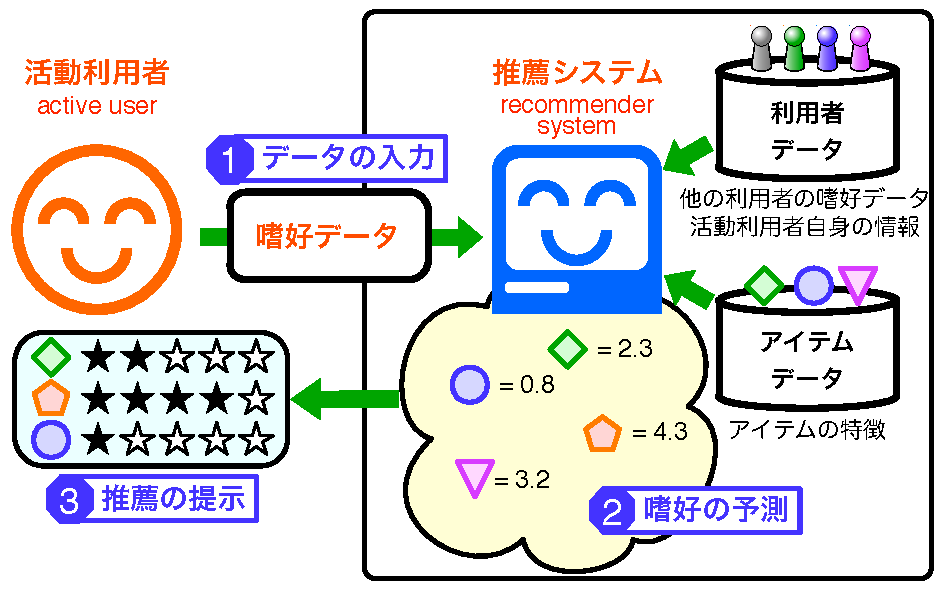
\includegraphics[width=0.8\fullwidth]{oipmodel.pdf}
\caption{推薦システムの実行過程(O-I-Pモデル)}
\label{fig:oipmodel}
\end{figure}

ここまでは,推薦システムを分類し,設計にあたって考慮すべき事項について述べてきた.ここでは,推薦システムがどのように実現されるかを見てゆこう.
推薦システムは,図\ref{fig:oipmodel}のように,データの入力,嗜好の予測,そして推薦の提示の三つの段階で推薦を行う.
これは\term{O-I-Pモデル}{output-input-process model}\cite{sigchi:03:01}とも呼ばれる.以下,これらの各段階の概要について述べる.

\begin{description}[style=nextline]
\item[データの入力]
推薦システムを利用して,推薦を受けようとしている人を\term{活動利用者}{active user}と呼ぶ.
活動利用者は自身の\termmain{嗜好データ}{preference data}を推薦システムに入力する.
嗜好データとは,いろいろなアイテムについての関心や好みの度合いを数値化したデータである.
この嗜好データの代わりに,関心のあるアイテムについてのより具体的な記述を検索質問や批評として,活動利用者に入力させるシステムもある.
また,推薦には,他の利用者の嗜好データ,アイテムの特徴データ,活動利用者自身の情報,推薦の状況や目的なども利用される場合があり,これらの情報を収集する場合もある.この段階については\ref{chap:input}章で述べる.
\item[嗜好の予測]
活動利用者の嗜好データに加え,収集しておいた利用者の他の情報やアイテムの情報を利用して,活動利用者がまだ知らないアイテムへの,活動利用者の嗜好を予測する.
嗜好の度合いを数値として予測する手法や,単に好きか嫌いかの識別をするだけの手法がある.
実現手段としては,機械学習の手法を用いるものや,人手によるルールを用いるものがある.
この段階については概要を\ref{chap:process}章で述べ,各種のアルゴリズムを第\ref{part:algorithm}部で紹介する.
\item[推薦の提示]
予測した嗜好に基づいて,目的に応じた適切な形式で,推薦結果を活動利用者に提示する.
%@@@ 評価の章を作ったら修正
このために,\ref{sec:systemtarget}節や\ref{sec:recomtask}節のいろいろな目的に応じた表示形式の変更や,\ref{sec:recomtype}節の各種指標のバランスを調整するためのアイテムの選別や順位付けの変更などを行う.
この段階については\ref{chap:output}章で述べる.
\end{description}

%!TEX root =  main.tex
%!TEX encoding = UTF-8 Unicode
\chapter{データの入力}
\label{chap:input}

ここでは,推薦システムの実行過程の最初の段階である「データの入力」について述べる.
この段階では,活動利用者に自身の嗜好データを,推薦システムへ入力させる.
嗜好データとは,利用者の各アイテムへの関心や好みの度合いをを数量化したものである.
システムによっては,この嗜好データの代わりに,活動利用者に検索質問や批評を入力させるものもある.
この検索質問は,アイテムの特徴についての制約条件を具体的に記述したものである.
例えば,レストランの推薦システムで,価格帯や,和洋中の別などを具体的に指示するために「価格は6000円以下で,和食の店」といった形式の検索質問を入力する.
こうした検索質問は,情報検索やデータベースのクエリ検索の技術がほぼ転用できるので,ここでは,嗜好データについて述べる.
さらに,これら嗜好データや検索質問で表された,活動利用者の嗜好パターンの以外のデータも推薦システムは利用する.
このようなデータとして,活動利用者以外の利用者の嗜好データ,アイテムの特徴,利用者の年齢や性別などの情報,現在位置などの利用状況を示す情報などがあり,これらにつても述べる.
なお,嗜好データの収集全般については,文献\cite{jjsai:04:05}にまとめられている.
また,文献\cite{sigir:01:01}は,推薦システムの利用者へのアンケート調査結果に基づいて,入力インタフェースについての設計指針を示している.
アイテムについての情報は,利用者が評価するときに見えるようにしておくと,システムへの満足が高まると報告している.

\section{暗黙的と明示的な嗜好データの獲得}
\label{sec:getprefimpexp}
\index{嗜好データ}\index{preference data}

\begin{table}
\centering
\caption{嗜好データ獲得法の長所と短所}
\label{tab:getprefcomp}
\begin{tabular}{l@{\qquad}c@{\,:\,}lc@{\,:\,}l}\toprule
 & \multicolumn{2}{c}{明示的} & \multicolumn{2}{c}{暗黙的} \\\midrule
データ量       & × & 少ない & ○ & 多い \\
データの正確さ & ○ & 正確 & × & 不正確 \\
未評価と不支持の区別 & ○ & 明確 & × & 不明確 \\
利用者の認知   & ○& 認知 & ×& 不認知\\
\bottomrule
\end{tabular}
\end{table}

まず,嗜好データを獲得するアプローチは,おおきく暗黙的と明示的の二種類に分けられる.
明示的な獲得とは,利用者に好き嫌いや,関心のあるなしを質問し,利用者に回答してもらう方法である.
もう一方の暗黙的な獲得とは,利用者の行動をから,利用者の嗜好や関心を推察することで嗜好データを得る方法である.
例えば,購入したり,閲覧したりしたアイテムには,利用者は関心があるとみなしたりする.

まず,二つの嗜好データの獲得法を比較する.
これらの獲得法の長所と短所を表\ref{tab:getprefcomp}にまとめた.
データ量については,利用者の嗜好の予測には統計的な方法が用いられるので,予測を正確にするにはより多くのデータを収集できた方が有利となる.
しかし,質問に答えるといった手間を利用者は嫌うことが多いため,明示的な獲得では多数のデータの収集は難しい.
よって,これらの点では暗黙的な手法が有利である.

データの正確さについては,暗黙的な獲得では,誤ってクリックしてしまったとか,人に頼まれて購入したなどの理由で,本当は関心がないものも,関心があるとみなされてしまう場合がある.このため,収集されたデータの正確さにおいては明示的な獲得が優れている.

利用者に明示的に評価してもらう場合では,アイテムを利用者が評価したかどうかはもちろん明確である.
しかし,暗黙的な評価では,利用者がそのアイテムに対して積極的な行動をしなかったことをもって,そのアイテムへの不支持とみなす場合がある.
例えば,閲覧しなかったアイテムは好きではないとみなしたとする.
このとき,アイテムについて未評価であることと不支持であることの区別ができない.
場合によっては,閲覧していないために,利用者が好むアイテムを嫌いだとシステムがみなすこともある.

最後の利用者の認知とは,利用者が自分の嗜好データをいつ,どのように取得されたかを知っているかどうかということである.
システムが提示した推薦は,利用者がその根拠を把握していた方が受け入れられやすい.
暗黙的な獲得では,嗜好データを意識的に入力していないので,推薦が根拠なくなされたもののように感じられやすく不利である.

\section{明示的な獲得}
\label{sec:explicitrating}
\index{明示的評価}\index{explicit rating}

アイテムを利用者に提示し,利用者にそのアイテムに対する好みの度合いを答えてもらう明示的な嗜好データの獲得について詳細を述べる.

\subsubsection{評価の動機付け}

明示的な獲得法では,利用者はアイテムを評価することを面倒だと思うので,暗黙的な方法に比べて多数の嗜好データを集めにくいと述べた.
\cite{sigir:01:01}では,利用者は推薦の精度が向上するなど,評価付けによるメリットが明確であれば,ある程度の手間をかけて評価付けをするとの調査結果を報告している.
よって,利用者に評価をさせるような動機付けは重要である.

自身への推薦の精度を向上させるということは,利用者にとって主な動機付けとなる.
だが,管理者が想定するようなこの動機以外にも,自分の意見の表明をするためや,他の利用者の手助けになるということを動機とする場合もある\cite{jacm:04:01}.
これらの動機は,利用者の評価数の順位の公開などによって喚起することができる.
さらに,明示的にインセンティブを与えることも考えられる.
文献\cite{ieeem:07:05}は,情報検索の結果の順位付けに,他の利用者の評価を利用する,一時的個人化の推薦システムを提案している.
このシステムでは,市場の考えが導入され,検索結果を閲覧するには,ポイントの支払いが必要である.
閲覧する文書の,被評価数が多く,評価が高いほど多くのポイントを支払う必要がある.
一方,ポイントは,検索した結果を評価することで獲得でき,被評価数が少なく,高い評価をすると獲得ポイント数は増える.
すると,検索をするために,検索結果の評価をする必要が生じるため,積極的な評価付けが期待できる.

\subsection{採点法と格付け法}

利用者が好みの度合いを答えるには,それを測る尺度が必要になる.
好みの度合いを表す尺度として,$0\sim5$ や$-3\sim+3$ のような数値尺度を使う\term{採点法}{scoring method} や,上・中・下 や 適合・不適合 などの順序付カテゴリ尺度を使う\term{格付け法}{rating method}\cite{j:0036}が良く利用されている.
こうした方法は人間の聴覚や味覚などを定量的に計測する官能検査(sensory test)の分野で研究されてきた\cite{jb:016:00}.
採点法や格付け法は,単純な入力フォームを用いて,比較的多数のアイテムに対する嗜好データを得られることが利点である.

これらの方法を使ううえでの注意点を幾つか述べておく.
%まず,尺度の段階の数は,利用者が真に要求している嗜好の段階数と等し
%いことが望ましい.
文献\cite{sigchi:03:02}では,利用者は評価尺度の目盛りが細かい方を好む傾向があること,さらに,細かい評価で予測精度が向上することはないが悪くもならないことを報告している.
よって,目盛りは細かめに設定することを推奨している.
さらに,${-}3$〜${+}3$の尺度で,中立の$0$を抜いた尺度を使うと,中立の評価の多くは弱い肯定的な評価$+1$に移されること,予測評価値を見せながら評価させると,利用者はそれに「引きずられた」評価をすることも報告している.
\ref{sec:recomtask}節で述べた適合アイテム発見を目的とする場合,目的に適合/不適合の2段階でも十分な場合が多いが,評価閲覧タスクでは,どれくらい不要なアイテムを除外したいかは利用者次第なので,より詳細な多段階の尺度を用いる方が良いだろう.
次に,質問の仕方にもいろいろな配慮をすべきである.
例えば,採点法では等間隔の尺度を連想させるように,等間隔の目盛りを見せるなどの工夫がある.これらの配慮については中森の\cite{jb:022:00}を参考にされたい.
%@@@ recsys:11:11:01

\subsection{評価値の揺らぎや偏り}

採点法や格付け法は大量の嗜好データを比較的に容易に得られるので多用されてきたが,当然ながら欠点もある.
先に,明示的な獲得は暗黙的な獲得と比べてより正確に利用者の嗜好を評価できると述べた.
だが,絶対的には不正確さや揺らぎがある.
真の嗜好の度合いは,脳の活動を直接観測するなどすれば将来的には計測できるであろうが,現在のところは厳密には計測できない.
そのため,揺らぎがあるかどうかの直接的な証明はできない.
よってここでは,採点法や格付け法によって計測した評価値が,真の評価値と乖離している間接的な証拠と,その乖離の原因を示す.

まず,評価値の揺らぎの証拠を示す.
官能検査の研究では,たとえ被験者が同じ評価値を与えていても,人によって嗜好の強さが違っていたりとか,時間がたつと一貫性が保たれなくなる問題があることが経験的に知られていた\cite{lncs:04:01}.
ソムリエなど訓練された被験者が,同一セッション内,すなわち,時間をあけずに連続して評価した場合でなければ,尺度を一定に保つことは難しいとされている.
嗜好データについても,一度映画を評価付けしたあと,6週間後にもう一度同じ被験者に同じ評価付けさせると,二つの評価値の間の相関は
0.83であったとの報告がある\cite{sigchi:95:01}.
文献\cite{sigchi:03:02}でも同様の報告がされている.
同一セッション内でも,寿司の嗜好について採点法で尋ねたのち,無関係な質問を幾つかしてから,下記の順位法で再び同じアイテムについて嗜好を質問すると,68.3\%の被験者の回答に不一致が観測された\cite{jpublist:043}.
これらの実験結果は,嗜好データには揺らぎがあることを示している.
他に,代表的な映画評価データにおいて,いろいろな工夫をしても,平均絶対誤差(MAE)を5段階尺度で0.73の「魔法の壁 (magic barrier)」より小さくできないことから,評価値そのものに揺らぎがあることが示唆されている\cite{jacm:04:01}.
以上のように,絶対的な評価値を使う採点法や格付け法では,被験者は,質問時期の違いなどにより揺らぎが生じるといえるだろう.

\begin{figure}
%(a) GroupLens   5.6  10.8  26.1  34.9  22.6
%(b) Amazon.com  7     5     8    20    60
%(c) 寿司        7.9   9.1  22.6  22.7  37.5
\centering
\subcaptionbox{MovieLens \cite{misc:129}\label{fig:prefdist:a}}%
{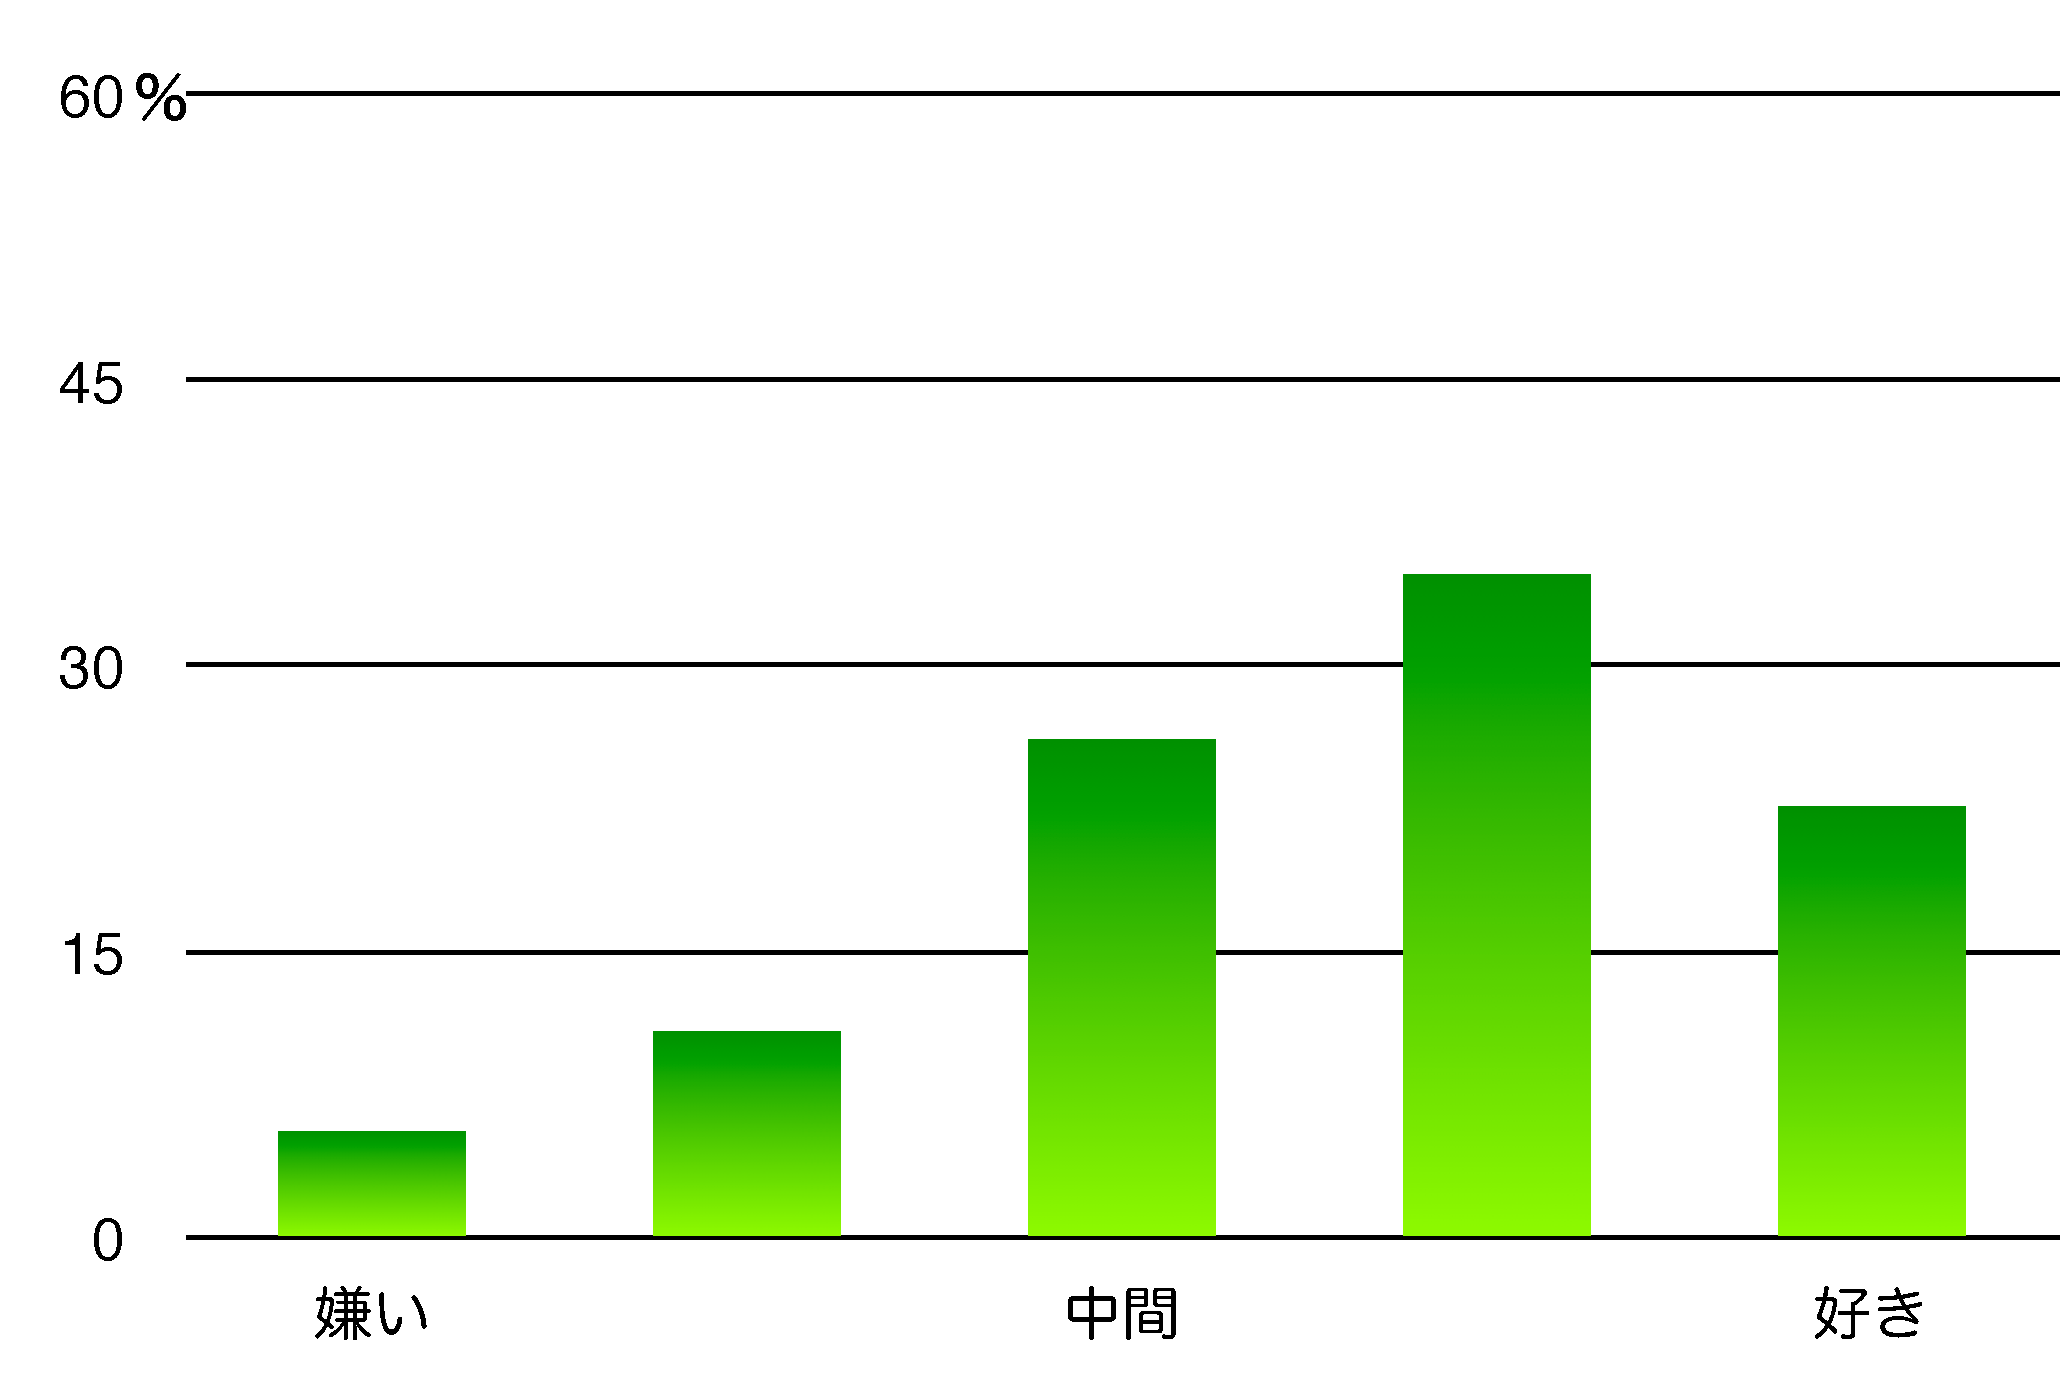
\includegraphics[width=0.6\linewidth]{rating-score1.pdf}}\\\medskip
\subcaptionbox{Amazon.com \cite{misc:007}\label{fig:prefdist:b}}%
{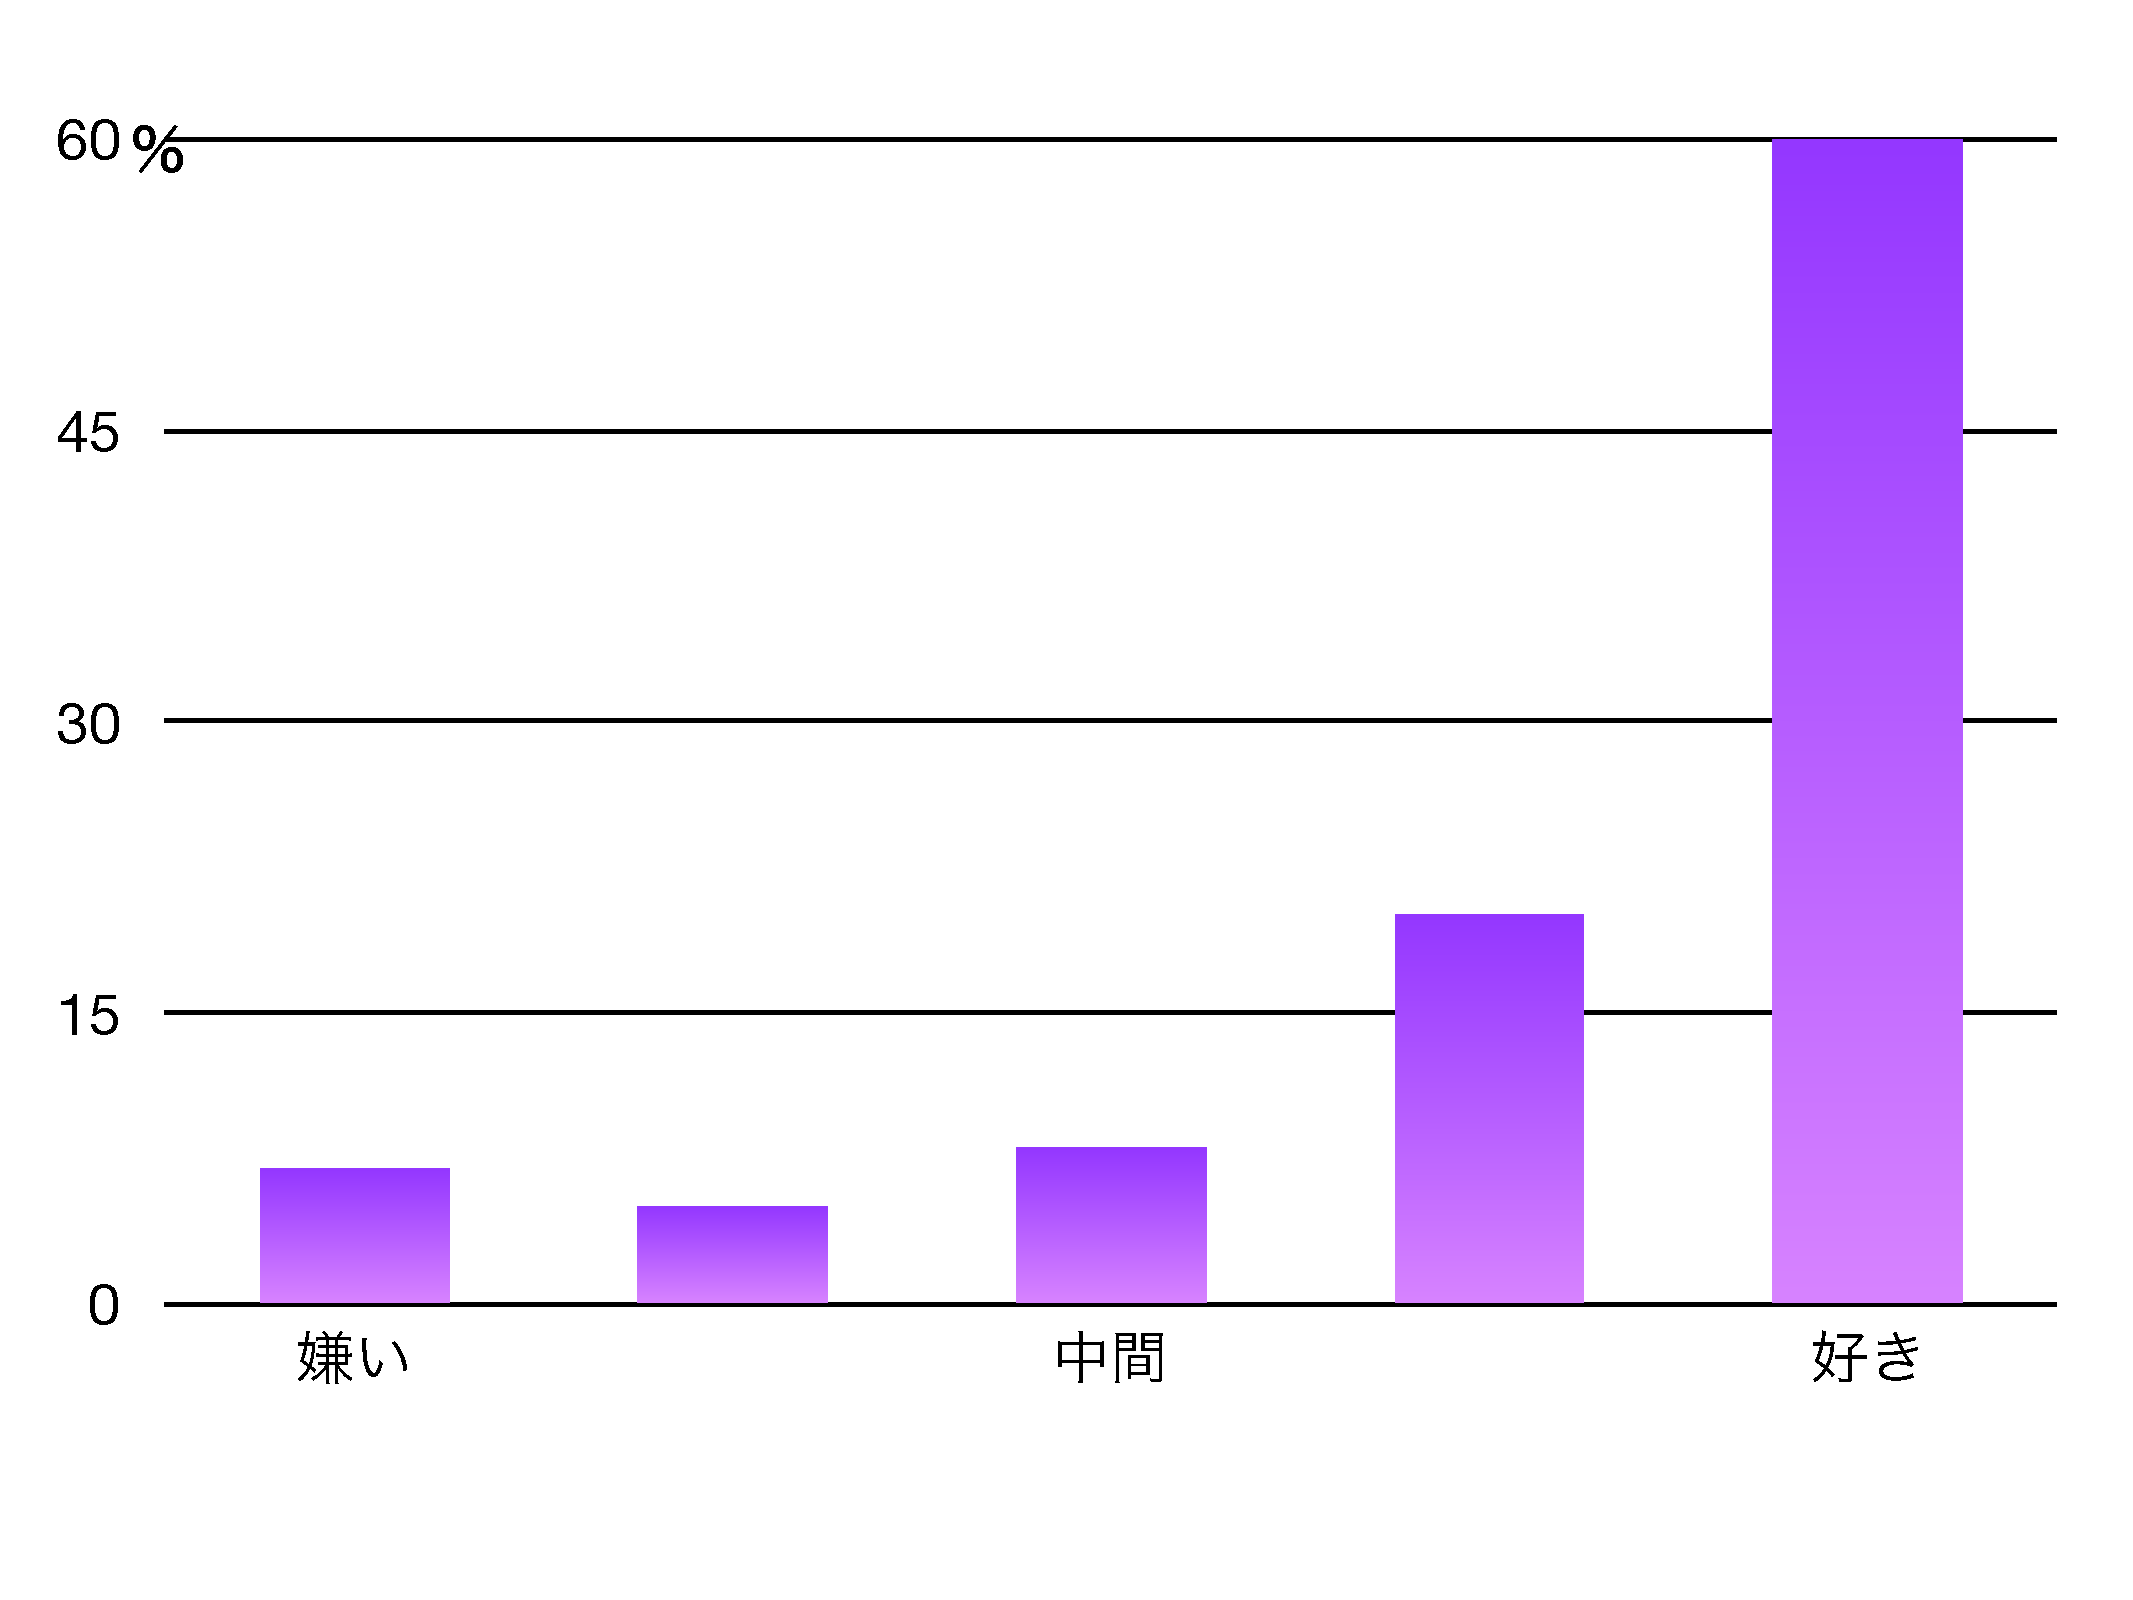
\includegraphics[width=0.6\linewidth]{rating-score2.pdf}}\\\medskip
\subcaptionbox{寿司 \cite{misc:140}\label{fig:prefdist:c}}%
{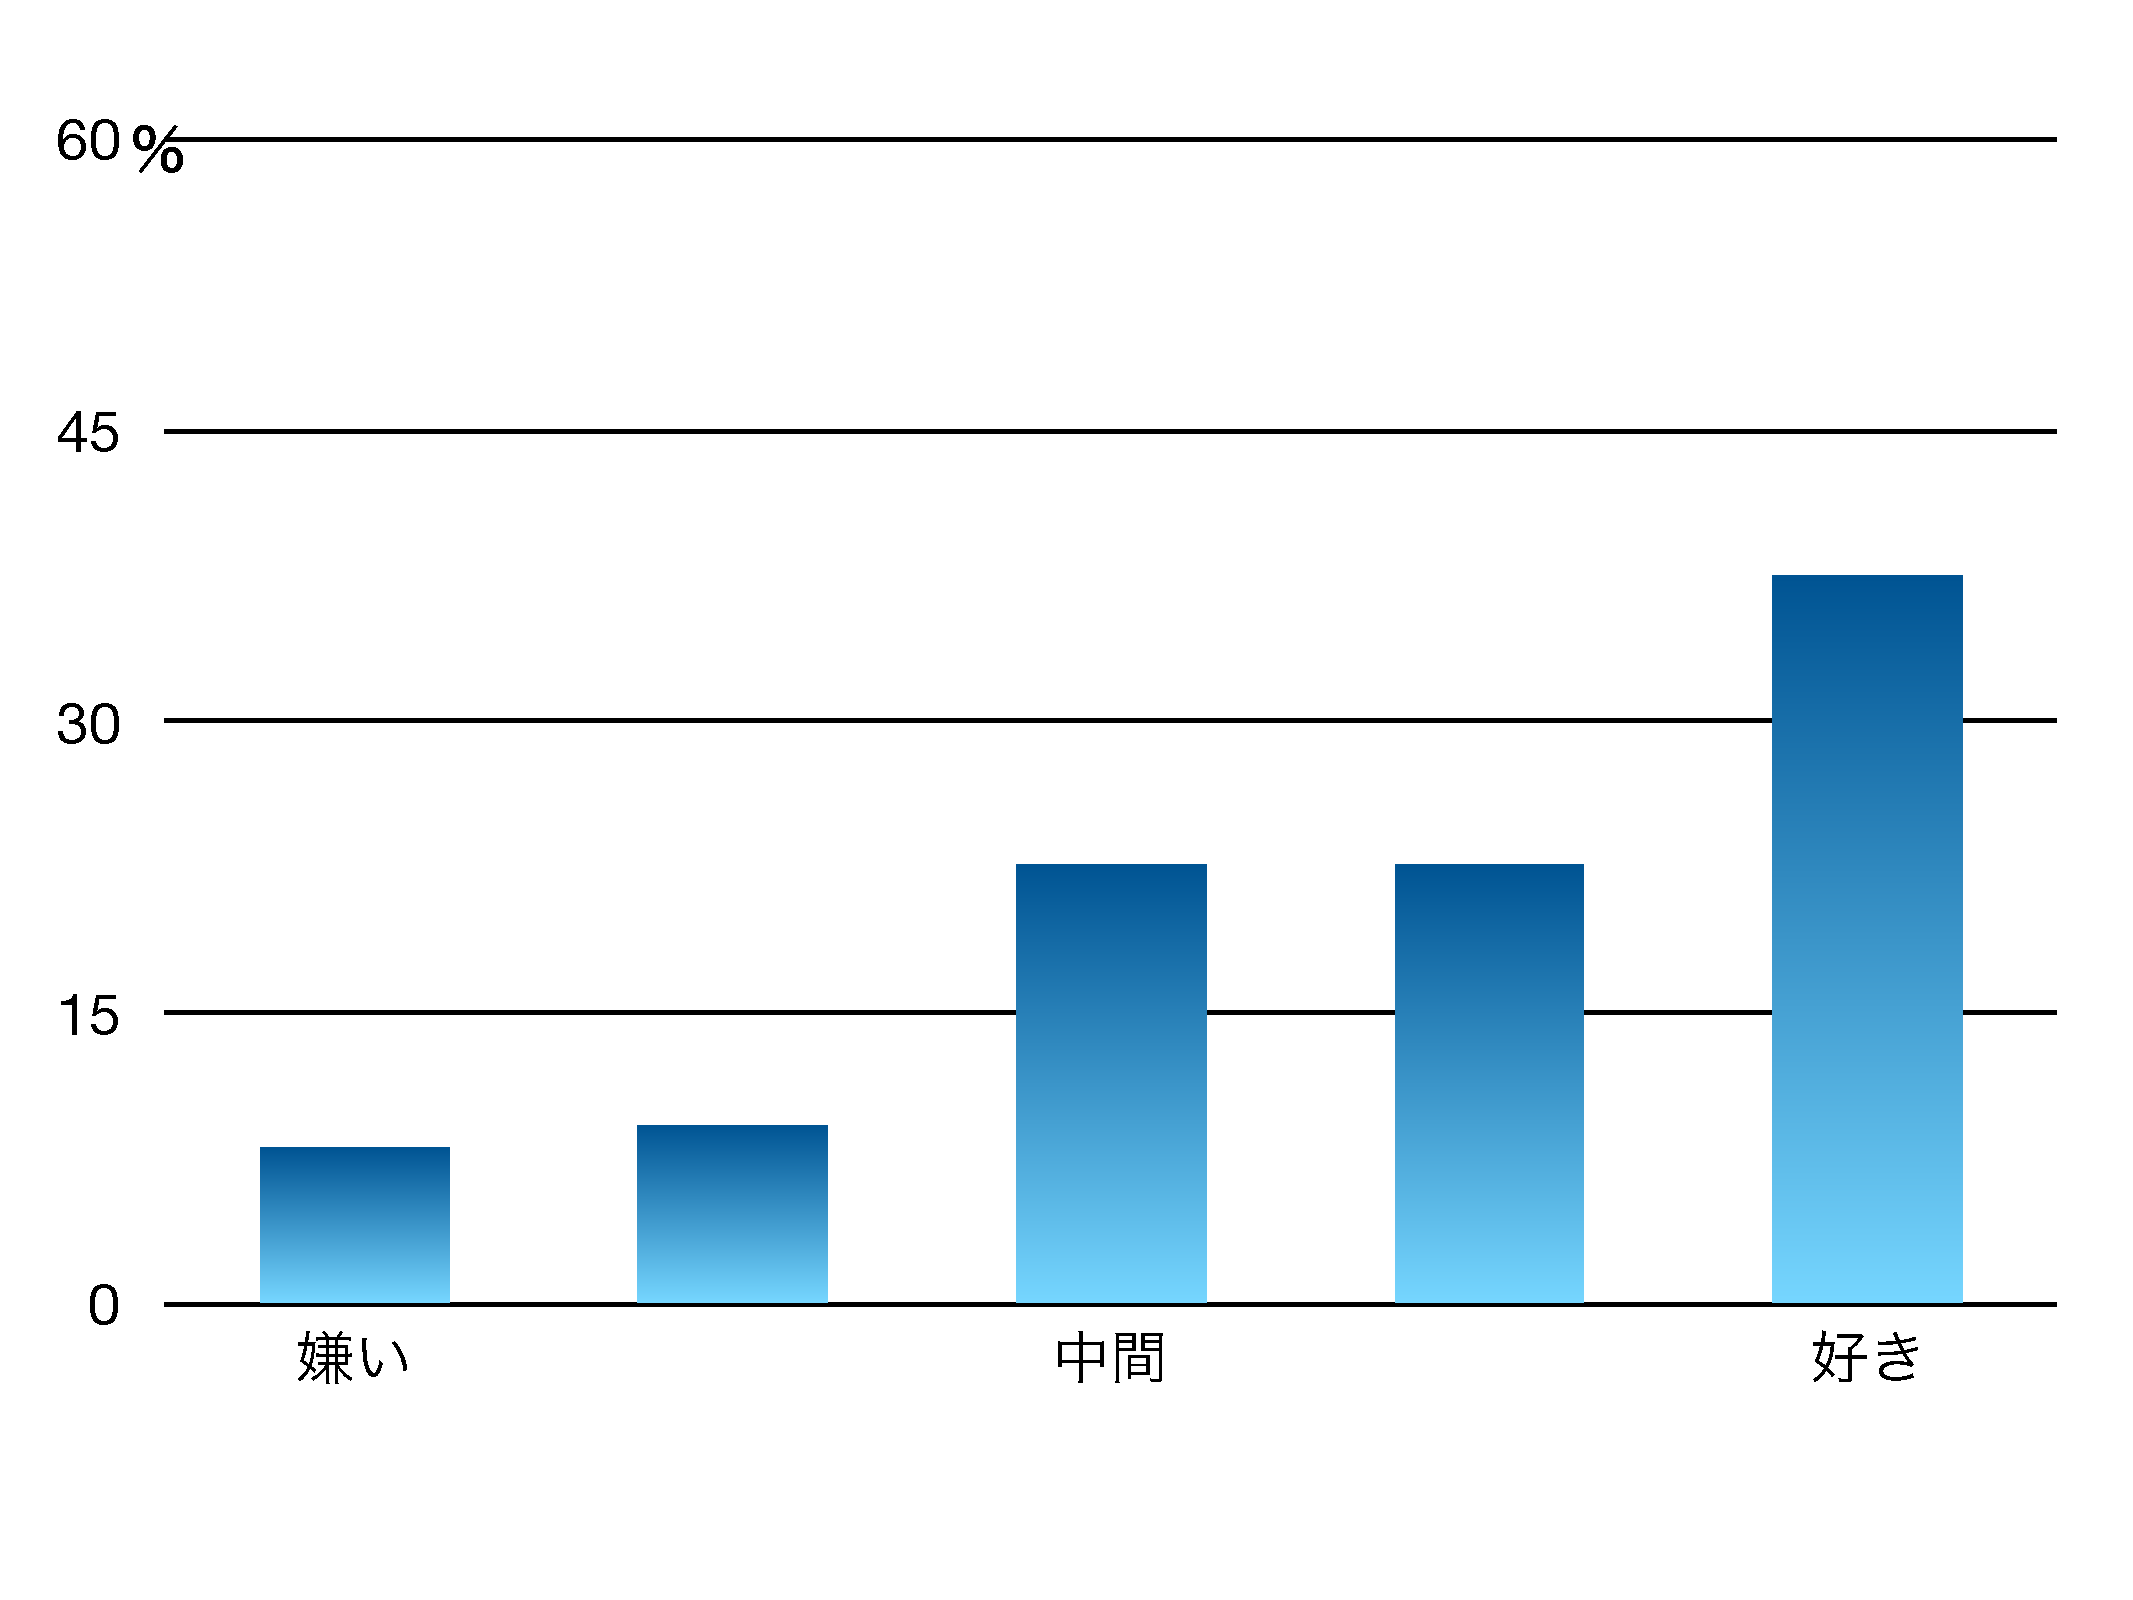
\includegraphics[width=0.6\linewidth]{rating-score3.pdf}}
\caption{アイテムへの評価値の分布}
\label{fig:prefdist}
\end{figure}

次に,評価値の偏りについて述べる.
図\ref{fig:prefdist}に,5段階の採点法を用いた3種類の嗜好データの,評価値の分布を示す.
それぞれ,\subref{fig:prefdist:a}~MovieLensの100万要素のデータ集合\cite{misc:129},\subref{fig:prefdist:b}~電子商取引サイトAmazon.com\cite{misc:007},\subref{fig:prefdist:c}~寿司の嗜好調査\cite{misc:140,epublist:064}での分布である.
どのデータでも,『好き』の方へ明らかに偏っている.
この偏りの原因には,サンプリングと真の嗜好からの乖離の二つが考えられる.
サンプリングの偏りの原因として,図\ref{fig:prefdist:a}や\subref{fig:prefdist:b}では,利用者が,関心がある選択的にアイテムを評価していることや,図\ref{fig:prefdist:b}や\subref{fig:prefdist:c}では,市場の淘汰を受けて人気のあるアイテムのみが評価候補となっていることが挙げられる.
このようなサンプリングの偏りは,\ref{sec:prederr}節で指摘したように,予測誤差の正確な評価を妨げる.
真の嗜好から乖離する理由としては,利用者個人がもつ心理効果の影響が考えられる.
例えば,過剰な酷評は社会的通念的に良くないとの考えをもつ人には,全体的に評価が高くする寛大効果 (leniency effect)が見られ,あいまいな判断や質問では中心のスコアを選びやすい中心化傾向 (central tendency)などが生じる\cite{jb:026:00}.
さらに,質問の仕方による影響も考えられる.
例えば,尺度の一方だけが連続して選ばれるように質問を配列すると偏りが生じる場合がある\cite{jb:022:00}.
%例えば,5を選び続けると,本当は4でも5と答えてしまったりする.
しかし,推薦システムでは,推薦結果の提示と嗜好データの収集を兼ねるため,利用者が好むと予測される順にアイテムを並べ評価付けさせることがよく行われる.
すると,高い評価値が高頻度で連続してしまう.
このように,設計上の制限により,偏りを生じるような質問の仕方をしてしまうという問題もある.

\subsection{順序の利用}

そこで,採点法や格付け法以外の調査方法の利用が考えられる.
文献\cite{sigir:99:02}では,利用者の類似度評価においてスコアの順位関係だけを考慮することや,利用者ごとの平均評価値を0に正規化することで予測精度が向上することを報告している.
このことは,採点法で得た評価値の絶対的な値ではなく,相対的な大小が重要であることを示唆しているといえるだろう.
また,採点法や格付け法で得られる量は,本質的には大小関係にのみ意味がある順序尺度\cite{eb:036:00,jj:015}であると指摘されている
\cite{jb:022:00}.
そこで,好きなものから嫌いなものへ順に,複数の対象を並べるという\term{順位法}{ranking method}を利用する「なんとなく協調フィルタリング」
\cite{epublist:039,epublist:064}を神嶌は提案した.
少なくとも調査したデータにおいて,順位法の採用で予測精度が向上した.
ただし,順位法にも問題点がある.
同時に多数のアイテムを整列するのは難しいので,大量の嗜好データをまとめて得ることは難しい.また,評価は常に相対的で,絶対的な評価は得られない.そのため,相対的に良いものを選ぶような意志決定には役立つが,絶対的な評価が求められる評価閲覧タスクなどには向かない.

官能検査の調査方法としては,取り出したアイテム対のどちらが良いかを指定する一対比較法(paired comparison)や,幾つかの候補の中から最良のものを指定させる択一法 (choice method) などもある.
これらの方法についての研究は著者はまだ知らず,今後の研究が待たれる.

\section{暗黙的な獲得}
\label{sec:implicitrating}
\index{暗黙的評価}\index{implicit rating}

暗黙的な嗜好データの獲得では,アイテムに関連した,利用者の行動に基づいて,そのアイテムについての嗜好を判断する.
利用者があるアイテムを閲覧したり,購入したりすると,これらの行動はそのアイテムへの潜在的な肯定を示していると考えられる.
また,購入は閲覧よりもより強い肯定を示すとも考えられる.
このような行動による潜在的な嗜好の強弱をNicholsは論じている\cite{misc:088,ej:048}.
強い嗜好を表すものから順に次のような行動を挙げている.
\begin{center}
\small
\begin{tabular}{llll}
1. Purchase & 2. Assess & 3. Repeated Use & 4. Save/Print \\
5. Delete & 6. Refer & 7. Reply & 8. Mark \\
9. Terminate Search & 10. Examine/Read & 11. Consider & 12. Glimpse \\
13. Associate & 14. Query & &
\end{tabular}
\end{center}
文献\cite{ieeem:07:01}では,閲覧,ビデオのプレビュー,購入の3種類の
行動それぞれを暗黙的な肯定入力と考え,それぞれの行動別に利用者間の
類似性を計算している.

他の暗黙的な獲得法として次のようなものがある.
推薦リストの上位からA, B, C,…とアイテムを閲覧してCを選んだとき,AやBを見たにも関わらずCを選択したことから,AよりC,BよりCを好むという相対的嗜好順序を得る方法\cite{kdd:02:01}が提案されている.
閲覧するという行為だけでなく,その時間を計測することで,より詳細な情報を得る方法などもある.
また,新たに入力装置を導入して,利用者の行動情報を収集し,そこから暗黙的に嗜好データを獲得する試みもある.例えば,マイクで収集した発話内容\cite{trjsai:07:01}や,アイカメラを使って求めた注視領域\cite{trjsai:07:02}などを利用する試みなどである.

\section{嗜好データのその他の要因}
\label{sec:getprefother}

嗜好データで推薦に影響するその他の要因を挙げておく.
利用者が初めてシステムを利用するときに,特定のアイテム群について明示的に質問して,嗜好データを集めることが考えられる.
全ての利用者が共通に評価しているアイテム群があると,\ref{chap:cf}章の協調フィルタリングでは利用者間の嗜好の類似性を評価しやすくなる利点がある.
しかし,音楽のようにその場で少し聞かせて評価できるようなものならよいが,映画などは見たことがないものは評価しにくい.
よって,こうした共通アイテム集合を利用できるかどうかは推薦するアイテムの種類に依存する.

評価したときの時間情報も利用できる.
服飾品のように流行の影響がある場合には,時間がたった嗜好データはあまり有効ではないだろう.
また時間の前後関係に依存する\ref{sec:timeseries}節のような嗜好の予測方法もある.
単純な好き・嫌いではなく,Zagatのレストランガイドのように,味・サービス・内装といった項目ごとに分けて嗜好データを収集することもできる.
こうしたシステムとしては\cite{ieeem:07:02}がある.

\section{嗜好データ以外のデータ}
\label{sec:featuredata}

嗜好データ以外の,推薦に利用されるデータについてまとめておく.

\subsection{アイテムの特徴}

アイテムを特徴ベクトルで記述したデータで,内容ベースフィルタリングでは必須である.
推薦対象がテキストである場合はBag-of-wordsモデルでtf-idf重み\cite{j:0021}が一般に使われる.この場合多数の特徴量が得られるが,個々の特徴の推薦への寄与は小さい.
一方,推薦システムの設計者が意図的に選択した特徴は,多数は得られないが,個々の特徴はより推薦に寄与する.
こうした特徴には,映画の場合では監督や制作年,ラーメンであればスープや麺の太さといったものが挙げられる.
このように,明確な特徴の他に,アンケート調査などで獲得した印象などを特徴にする場合もある.映画の例では「悲しい」や「楽しい」といった印象語への採点法による評価の平均評価値などを特徴量として利用できる.

\subsection{個人属性の特徴}

利用者の年齢や性別などの\term{個人属性情報}{demographic information}も利用できる\cite{ej:050}.
これらの情報は嗜好と関連があると考えられ,マーケティングにおいてもデータベースマーケティングとして利用されてきた\cite{dmkd:01:01}.
%活動利用者以外の嗜好データも利用するシステムでは,その利用者の推薦
%における重要度\cite{tjsai:04:09}なども利用できる.
個人属性の特徴があれば,新規利用者に対しても推薦が可能になる利点があるが,プライバシー問題の観点から,その収集が困難である問題がある.
この問題に対しては,データの利用目的を説明すること\cite{sigir:01:01}や,\ref{chap:privacy}章のプライバシー協調フィルタリングの導入といった対処がある.

\subsection{利用状況の特徴}

推薦システムを利用する状況の情報である.
レストランを利用する場合などでは人数や場所の情報は推薦の制約になる\cite{tjsai:06:01,trjsai:06:01}.
また,システム側のコンテキストとして,商品の在庫や納期の情報など,推薦時には考慮すべき情報である.

%!TEX root =  main.tex
%!TEX encoding = UTF-8 Unicode
\chapter{嗜好の予測}
\label{chap:process}

嗜好の予測とは,活動利用者の嗜好データや,アイテムの特徴を用いて,活動利用者の各アイテムへの関心や好みの度合いを予測することである.

嗜好の予測段階の実現方法は大きく二つに分類される.
レンタルビデオ店で,顧客が見たい映画を推薦する場合を考えてみよう.
一つは,ファンである監督,好みのジャンルを利用者に尋ねてその条件に合ったものを選ぶ方法である.
これを,検索対象の内容を考慮して推薦をするので\term{内容ベースフィルタリング}{content-based filtering}と呼ぶ.
もう一つは,映画の趣味が似ている知り合いに,面白かった映画を教えてもらう「口コミ」の過程を自動化する方法である.
他の人との協調的な作業によって推薦対象を決めるため,この推薦手法は\term{協調フィルタリング}{collaborative filtering}や社会的フィルタリング (social filtering)と呼ばれている.

\begin{figure}
%(a) GroupLens   5.6  10.8  26.1  34.9  22.6
%(b) Amazon.com  7     5     8    20    60
%(c) 寿司        7.9   9.1  22.6  22.7  37.5
\centering
\subcaptionbox{内容ベースフィルタリング(間接指定型)\label{fig:cfcbf:a}}%
{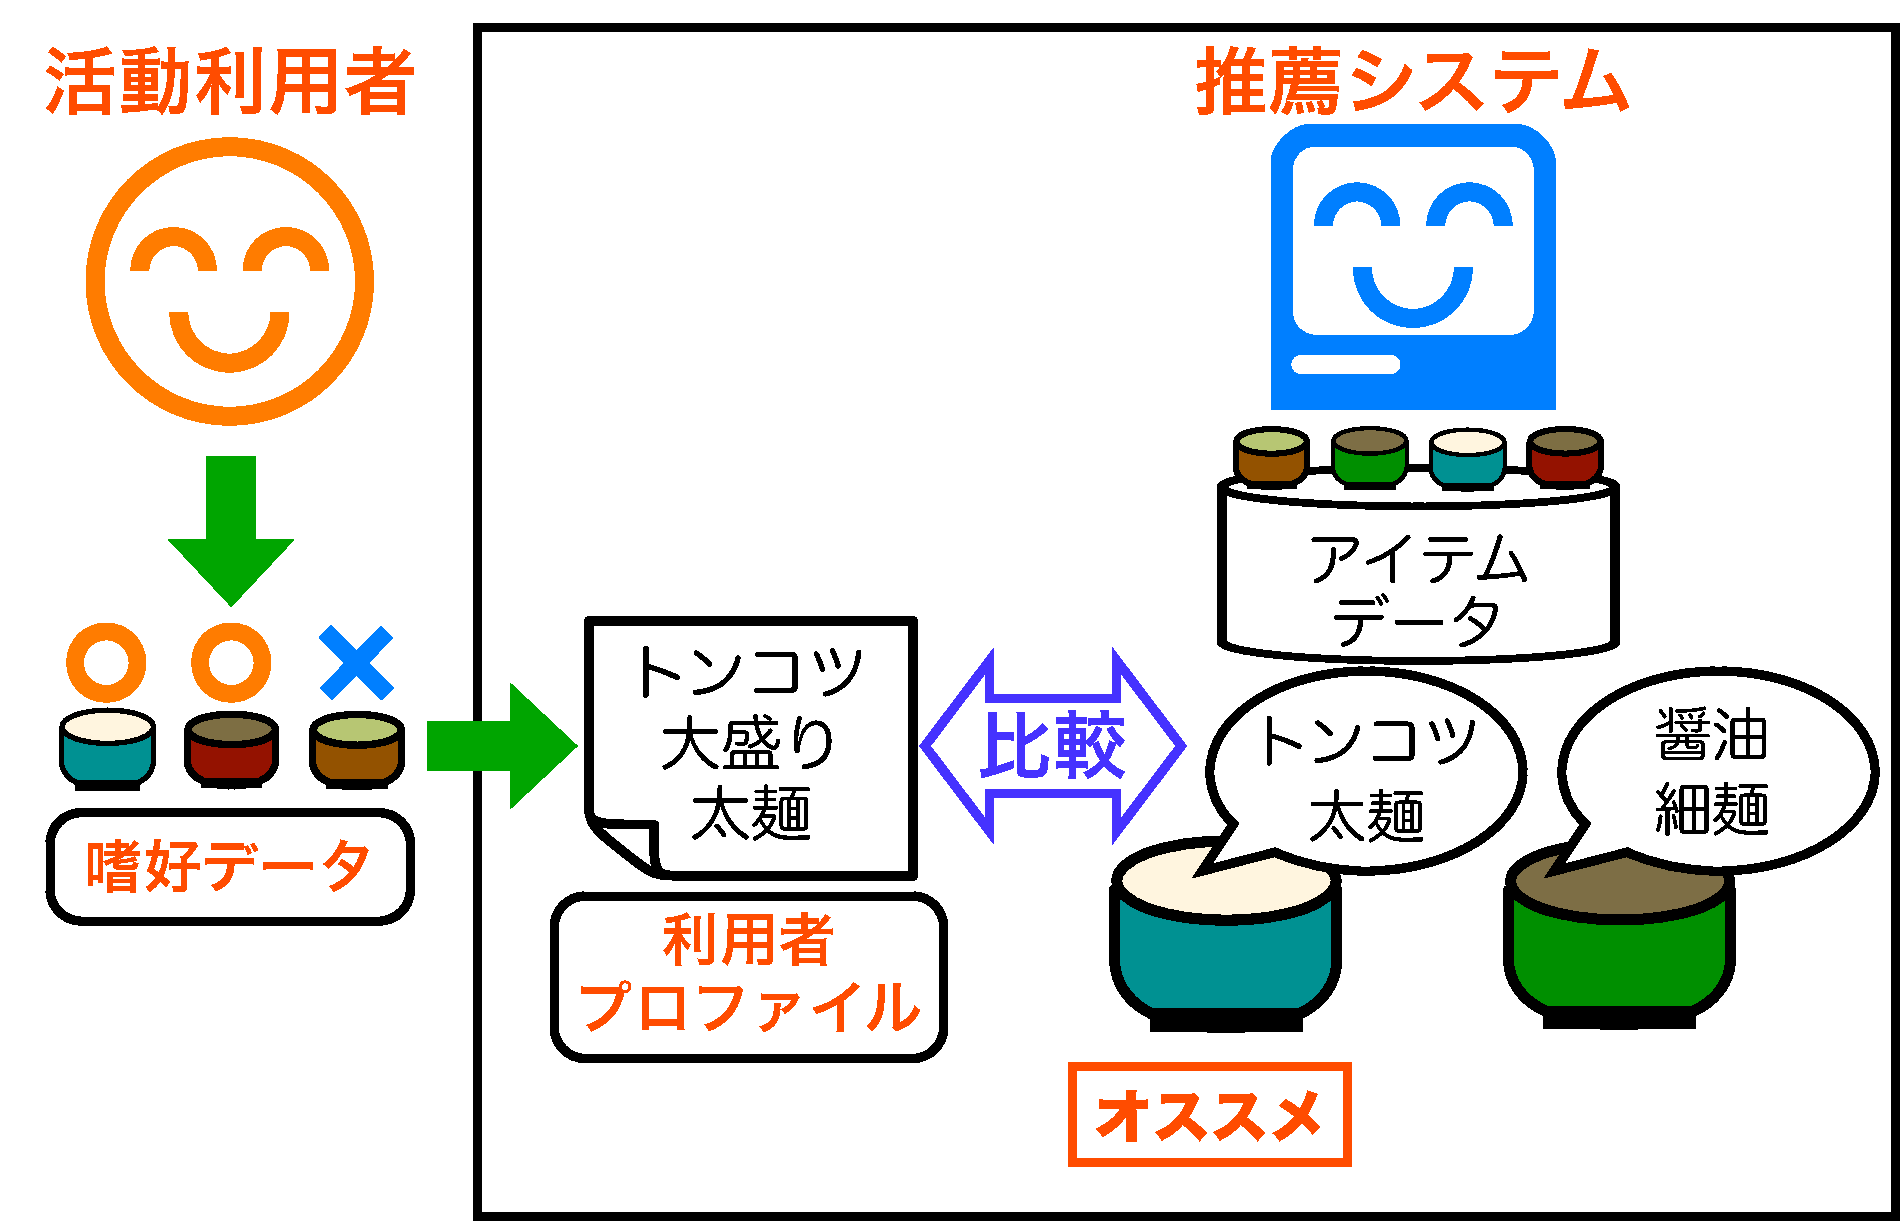
\includegraphics[width=0.6\linewidth]{rsyscategory-icbf.pdf}}\\\medskip
\subcaptionbox{内容ベースフィルタリング(直接指定型)\label{fig:cfcbf:b}}%
{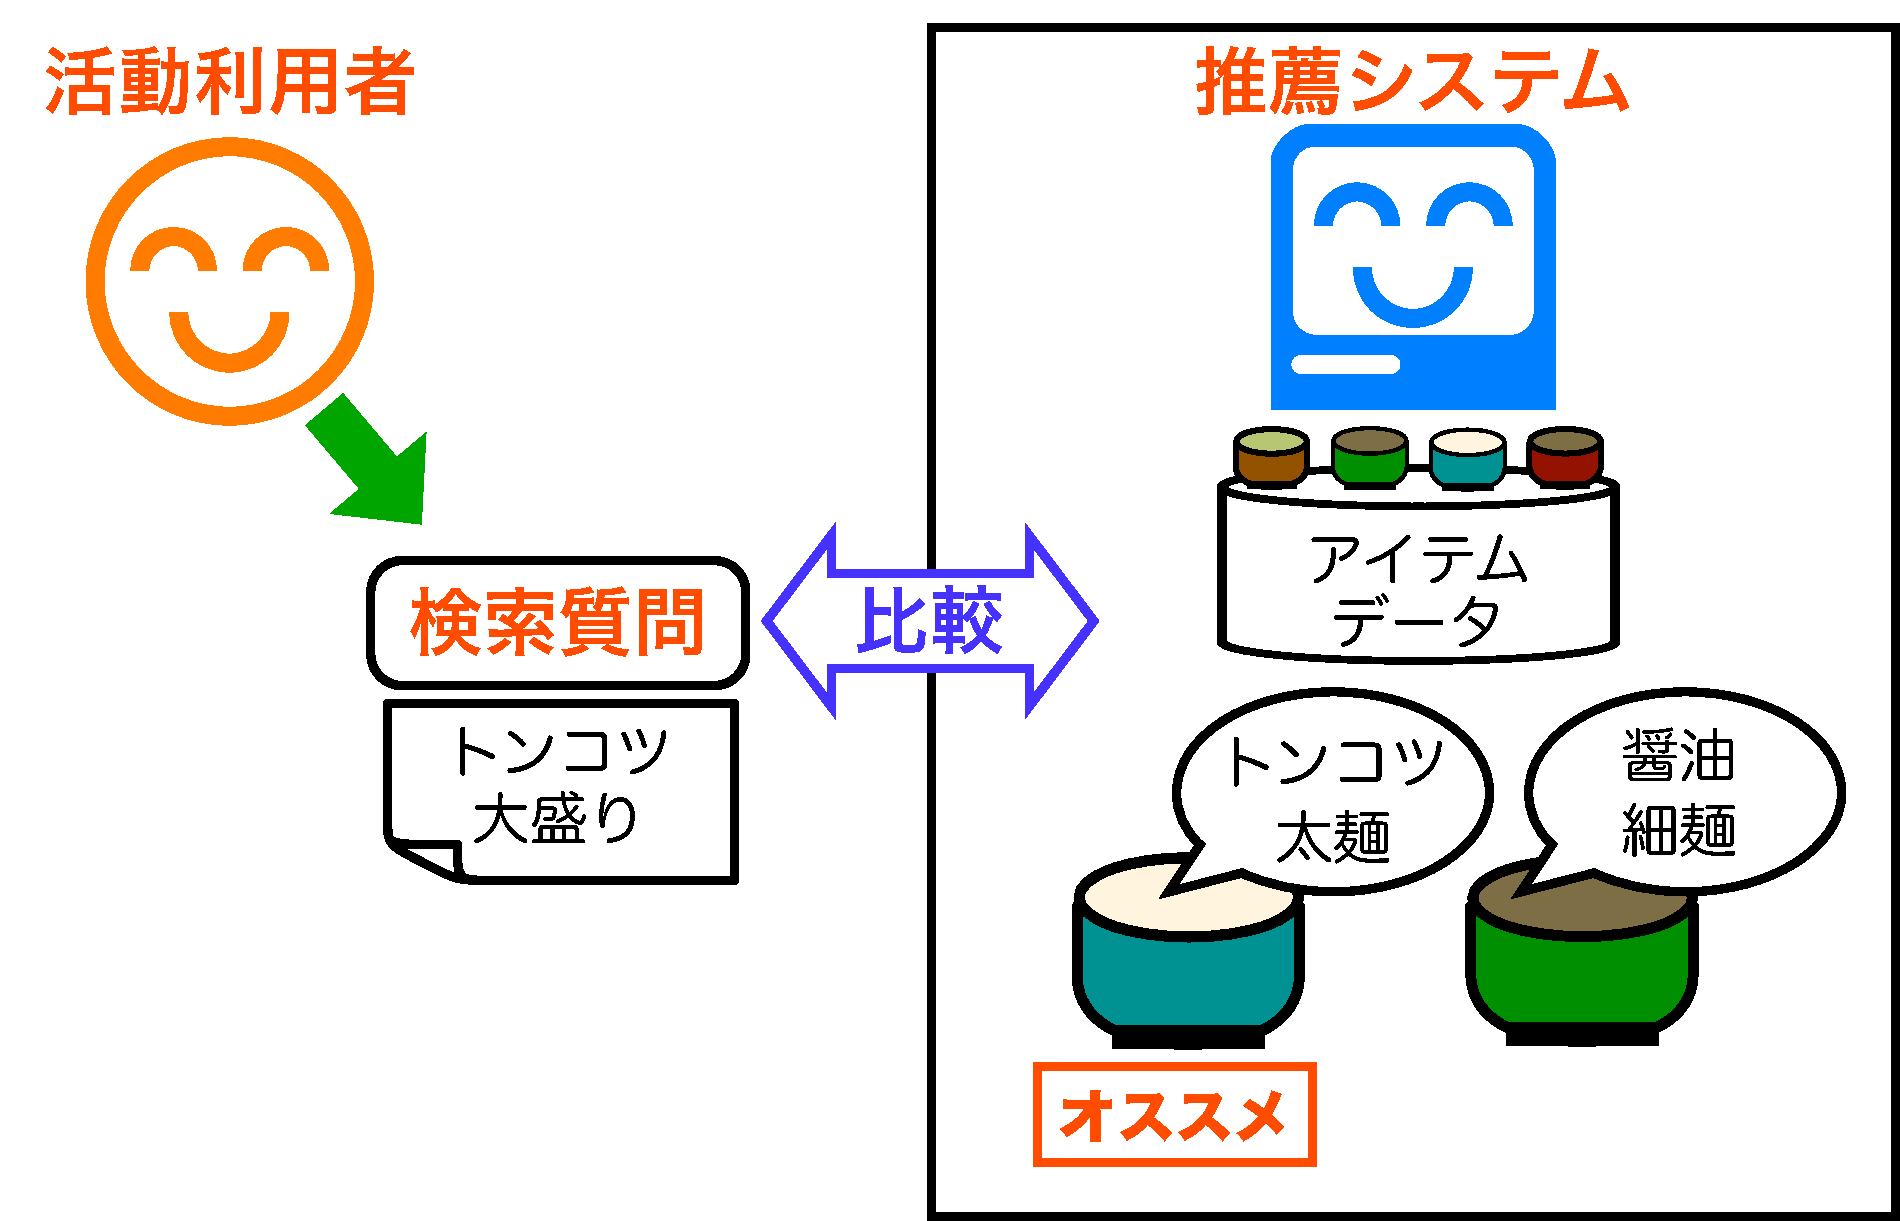
\includegraphics[width=0.6\linewidth]{rsyscategory-dcbf.pdf}}\\\medskip
\subcaptionbox{協調フィルタリング\label{fig:cfcbf:c}}%
{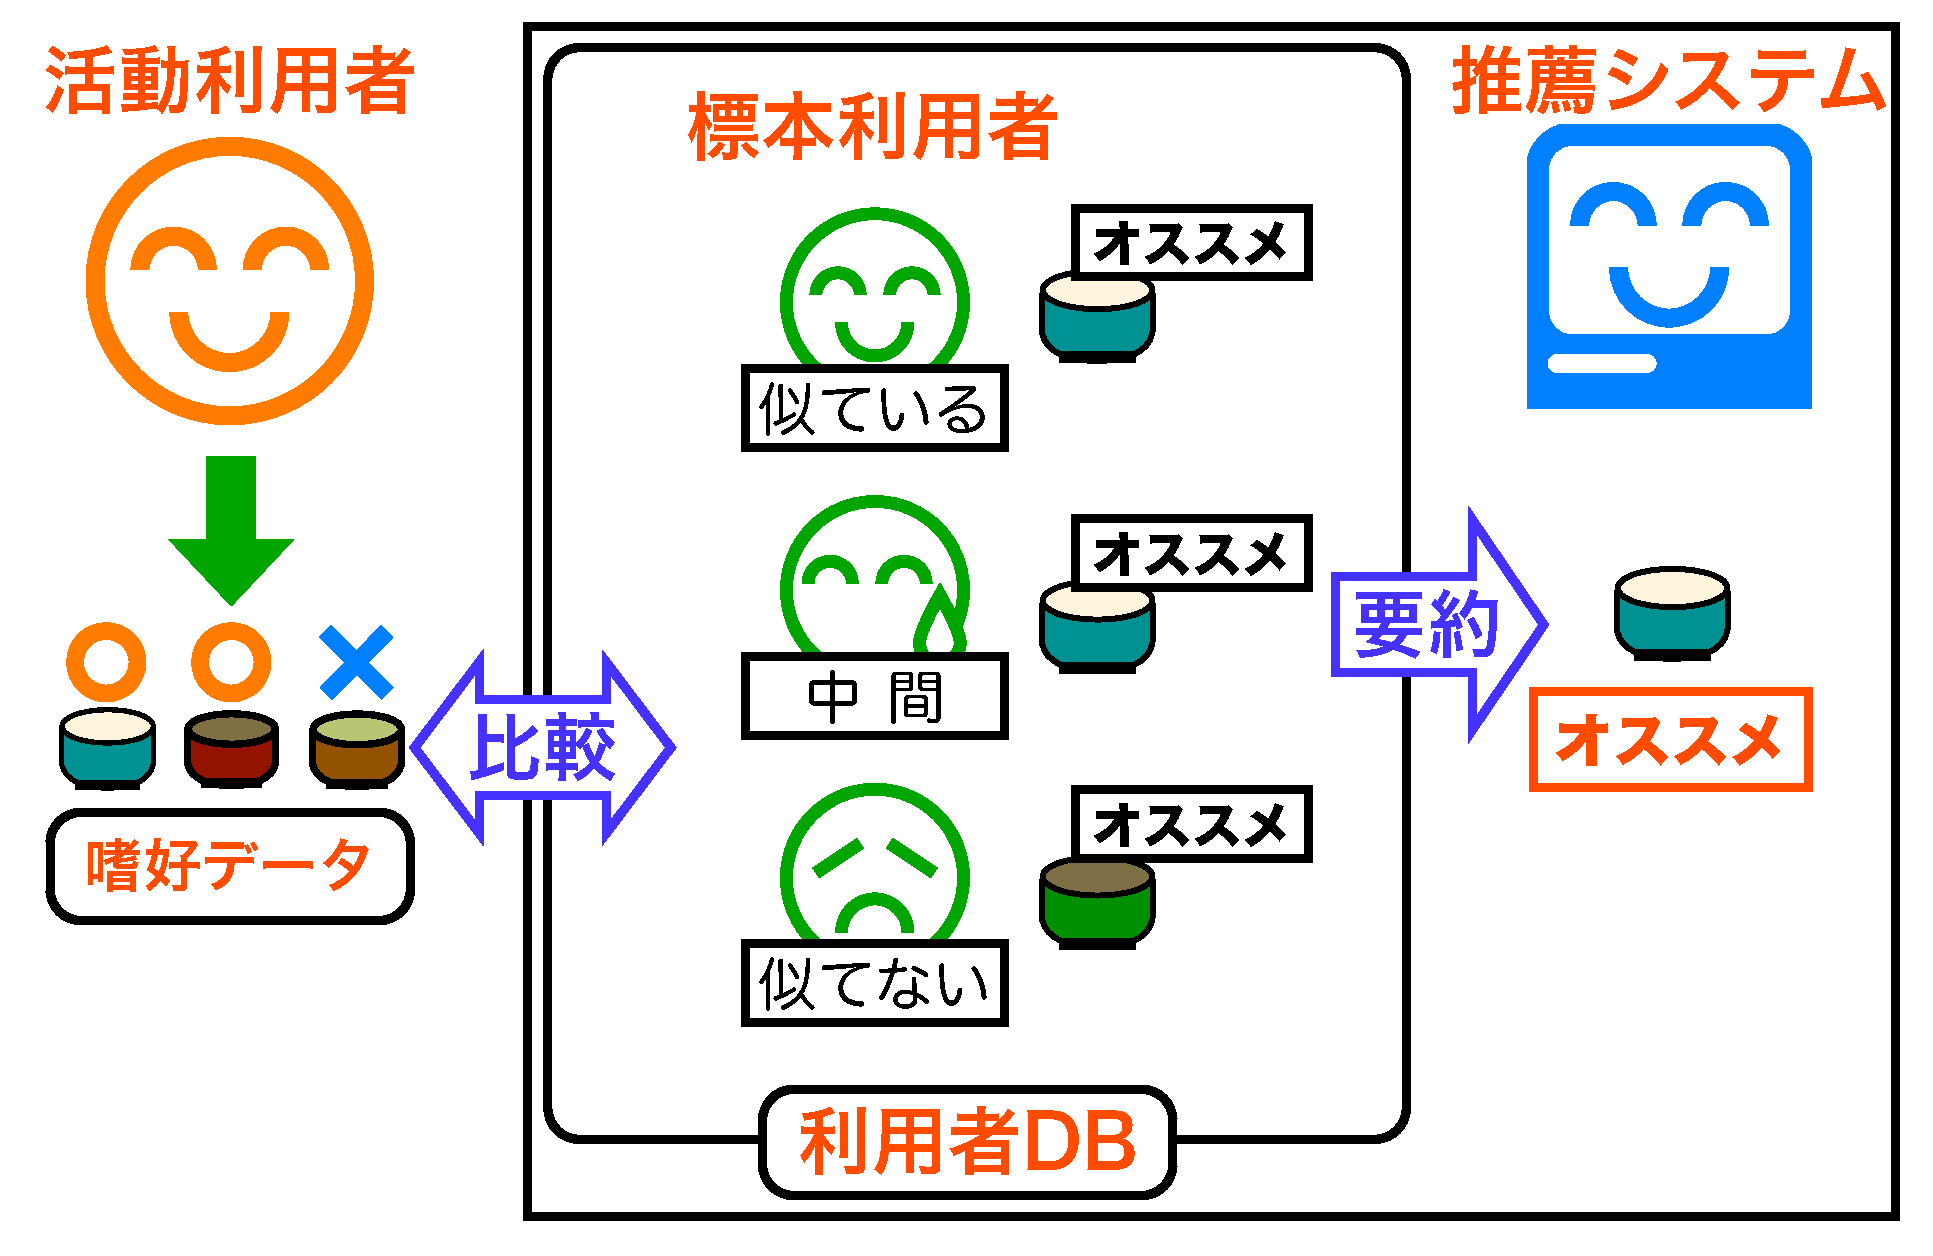
\includegraphics[width=0.6\linewidth]{rsyscategory-cf.pdf}}
\caption{内容ベースフィルタリングと協調フィルタリング}
\label{fig:cfcbf}
\end{figure}

現在では,どちらの方法にもいろいろな派生型が提案されているが,純粋な形では図\ref{fig:cfcbf}のように予測する.
内容ベースフィルタリング(図\ref{fig:cfcbf:a}と\ref{fig:cfcbf:b})では,アイテムの性質と利用者の嗜好パターンを比較して,利用者が好むと判断したものを推薦する.
このアイテムの性質は特徴ベクトルによって記述される.
特徴ベクトルとは,アイテムのいろいろ側面の性質を表す特徴を集めて,ベクトルの形にしたものである.
各特徴は,事前に定めた定義域中の値をとることで,そのアイテムの性質を表現する.
ラーメンの例を示そう.このとき,スープの種類,麺の太さ,価格といった特徴からなるベクトルでラーメンを表現する.
スープの種類という特徴は,トンコツ,醤油,塩のような定義域の値の一つをとり,価格という特徴では自然数がその定義域となる.
そして,ある特定のラーメン『トンちゃん』があるとすると
\begin{center}
\footnotesize
(スープの種類=トンコツ, 麺の太さ=細麺 ,…, 価格=650円)
\end{center}
といったベクトルで表現される.
こうした情報をいろいろなアイテムについて収集したものをアイテムデータと呼んでおく.
一方,利用者の嗜好パターンは\term{利用者プロファイル}{user profile}によって表す.
この利用者プロファイルを間接指定するシステムと,直接指定するものがある.
間接指定型(図\ref{fig:cfcbf:a})では,利用者のいろいろなアイテムに対する嗜好データ,すなわち,好き嫌いの度合いを定量化したデータを集める.
この嗜好データと,アイテムデータに基づいて,その利用者が好むアイテムの特徴のパターンを機械学習の手法でモデル化し,利用者プロファイルとする.
直接指定型(図\ref{fig:cfcbf:b})では,利用者が明示的に,自身が好むアイテムの特徴を表した検索質問(query)(批評(critique)ともいう)を入力する.
一般的な検索質問は「スープの種類は醤油で,価格は500円以下」といった,特徴に対する制約の形式だが,自然言語文などを扱えるものもある.
この検索質問はそのまま利用者プロファイルとして用いられる.
内容ベースフィルタリングでは,アイテムデータ中のアイテムの特徴ベクトルと,利用者プロファイルとを比較し,プロファイルに最も近い特徴ベクトルをもつアイテムを利用者が好むものと判断して推薦をする.

もう一つの協調フィルタリング(図\ref{fig:cfcbf:c})では,アイテムの性質は全く考慮しない.
その代わりに,システムが利用される前に,多くの利用者の,いろいろなアイテム対する嗜好データをデータベースに集積している.
このデータベースを\term{利用者データベース}{user database}(「利用者DB」と略す)と呼び,この利用者DBに嗜好データを登録している利用者を\term{標本利用者}{sample user}と呼ぶ.
さらに,今までの嗜好パターン,すなわち,どのアイテムを好み,どのアイテムを嫌うのかという傾向が類似している利用者は,これからも同じアイテムを好み,同じアイテムを嫌うであろうという仮定を導入する.
この仮定の下,活動利用者と,嗜好パターンが類似している標本利用者を見つけ,これらの標本利用者が好むものを活動利用者に推薦する.

なお,内容ベースフィルタリングは,いろいろな拡張が行われているので,厳密に定義するのは難しい.
文献\cite{ej:048}では,個人属性の特徴(\ref{sec:featuredata}節)などを用いず,アイテムの特徴のみを用いた,間接指定型の手法のみを内容ベースフィルタリングと定義している.
そして,上記の直接指定型にあたる知識ベース型や,デモグラフィックな特徴を使うものも,別の種類として細かく分類している.
しかし,細分化しても多種多様な手法を厳密に分類するのは実際には難しいので,本稿では,広義にとらえて,アイテムやデモグラフィックな特徴を利用するような方法は全て内容ベースフィルタリングとして扱う.
一方,これらの特徴を用いず,標本利用者の嗜好データのみを用いる方法を協調フィルタリングとしておく.

第\ref{part:algorithm}部では,協調フィルタリングと内容ベースフィルタリングの各種手法を順に紹介する.
さらにその後に,これら二つの手法を組み合わせるハイブリッド法について述べたのち,アルゴリズムの選択の指針について述べる.
これらの話題に移る前に,協調フィルタリングと内容ベースフィルタリングの長所と短所をまとめておく.

\section{内容ベースと協調フィルタリングの比較}
\label{sec:cfcbfcomp}

\begin{table}
\centering
\caption{協調フィルタリングと内容ベースフィルタリングの比較}
\label{tab:cfcbfcomp}
\begin{tabular}{l@{\qquad}>{\centering}p{6zw}>{\centering}p{6zw}p{0pt}}\toprule
%\begin{tabular}{l@{\qquad}cc}\toprule
 & 協調 & 内容ベース & \\\midrule
多様性 & ○ & × & \\
ドメイン知識 & ○ & × & \\
%疎なデータ & △ & × & \\
スタートアップ問題 & × & △ & \\
利用者数 & × & ○ & \\
被覆率 & × & ○ & \\
類似アイテム & × & ○ & \\
少数派の利用者 & × & ○ & \\
\bottomrule
\end{tabular}
\end{table}

協調フィルタリングと内容ベースフィルタリングの長所と短所を\cite{macm:97:02,ej:048}などに基づき表\ref{tab:cfcbfcomp}にまとめた.
以下,表中の各項目について詳しく述べる.

\subsection{多様性}
\index{diversity}\index{多様性}

\ref{sec:recomtype}節で述べた多様性・セレンディピティについては,協調フィルタリングが有利と言われている.
内容ベースフィルタリングでは,利用者自身が知っているアイテムの特徴に,推薦対象が制限されてしまうことが多い.
例えば,映画の場合であれば,過去に見たのと同じジャンルや監督の作品が推薦される.
さらに,類似した内容のアイテムを推薦し,それを利用者が受け入れることで,利用者プロファイルの偏りが一層強化される現象も生じる.
それに対して,協調フィルタリングでは,自身が知らないジャンルや監督でも,他の標本利用者の知識を通じて知ることができる場合がある.
そうしたときには意外性のある,すなわち,セレンディピティがある推薦ができるとされている.

\subsection{ドメイン知識}

協調フィルタリングの最も重要な長所は,アイテムの特徴,すなわち,アイテムの\term{ドメイン知識}{domain knowledge}を全く必要としないことである.
アイテムの特徴ベクトルの設計に伴う困難には次のようなことがある.
\begin{itemize}
 \item
アイテムの特徴についてのデータを集める手間やコストが必要になる.
仕様についてのデータベースが整備されている商品分野は書籍,CDなどに限られている.
たとえ整備されていても,食品の成分表などのように推薦という目的にはあまり役立たないものもある.
それ以外の分野ではデータベースの構築・更新コストが必要になる.
 \item
 アイテムのある性質を表す特徴がないために,適切な推薦ができないことがある.
 例えば,映画の推薦で,自分がファンであるカメラマンの撮る映画を見る利用者がいたとしても,映画の特徴ベクトルに『カメラマン』の特徴がなければ,内容ベースでは適切な推薦ができない.
%テキストを対象とするときは語の頻度がよく利用されるが個々の特徴の質
%は低い.その他,映画などでは,特徴を数十〜数百種類利用するこ
%とは一般に困難で,量的に制限される.このように,特徴の設計に
%は困難が伴う.
 \item
 どの特徴を採用するかということが,利用者の判断に影響を与える.
推薦アイテムの決定に利用された特徴は,利用者の意志決定でより重要視され,そうでない特徴は無視されるようになる副作用を生じることがある\cite{ec:029}.
 \item
 違う分野のアイテムを推薦することが困難である.
 例えば,ある映画が好きでも,内容ベース法では,そのサントラのCDを推薦することは難しい.
 なぜなら,映画とCDは,異なる特徴ベクトルで表現されているためである.
\end{itemize}

%\subsubsection{疎なデータ}
%
%\ref{sec:rsyslimit}節で述べたように,推薦システムが扱うデータは疎であ
%る.
%すなわち,推薦対象の数に対する,利用者一人あたりのアイテムに対する
%評価値の数は非常に少ない.
%内容ベースと協調のどちらにとっても疎なデータからの嗜好の予測は困難
%な問題である.
%だが,協調フィルタリングでは,活動利用者の嗜好データの他に,標本利
%用者の嗜好データも利用できる.
%一方,内容ベースでは,活動利用者の嗜好データのみに依存する.
%そのため,データが疎である問題は相対的に内容ベースの方でより一層深刻である.
%さらに
%内容ベースの方法では,推薦時に利用者の嗜好データを新たに要求するな
%どの対処方法がある.

\subsection{スタートアップ問題}

\term{スタートアップ問題}{start-up problem}(コールドスタート問題やランプアップ問題とも呼ぶ)は,2種類に分けられる.
一つは,新たにシステムを利用し始めた利用者(first raterやearly raterともいう)に対して適切な推薦をする難しさであり,もう一つは,推薦対象として新たにシステムに導入されたアイテムを推薦する難しさである.
前者については,協調フィルタリングでは,他の標本利用者との類似性を判定できないため良い推薦をするのは難しい.
間接指定型の内容ベースフィルタリングでも,利用者プロファイルが不完全になるためやはり難しい.
加えて,利用者本人の評価値しか利用できないので,問題がさらに深刻になることがある.
だが,直接指定型の内容ベース法では,自身の利用者プロファイルを直接記述するためこうした問題は生じない.
よって,観光地の案内端末での推薦など,同一利用者の継続的な利用があまりない状況では,直接指定型の内容ベース法を採用すべきである.
一方,継続的な利用がなされるならば,嗜好データの蓄積に伴って予測精度が向上する協調フィルタリングや間接指定型の内容ベースフィルタリングがよいであろう.

一方,後者の新規アイテムに対する問題については,内容ベースフィルタリングが優れている.
内容ベースフィルタリングでは,利用者プロファイルがあれば,新規のアイテムでも,その特徴ベクトルを手がかりに,全く問題なく推薦ができる.
しかし,協調フィルタリングでは,標本利用者の評価を利用するので,まだ誰も評価していない新規のアイテムは,推薦を予測する手がかりがなく,そのアイテムに対する活動利用者の好みを判断できない.
以上のことから,商品が頻繁に入れ替わるような場合は,内容ベースフィルタリングが有利である.

\subsection{利用者数}

内容ベース法の場合は,たとえシステムの利用者が一人であっても推薦は可能である.
一方,協調フィルタリングは,他の利用者の意見を参照するので,利用者数がある程度なければ実行できない.
また,利用者が他にいない状況では,適切な推薦もできないため,新たな利用者の増加も難しい.
そのため,電子商取引サイトでのポイントの配布といったインセンティブや,暗黙的な方法で自動収集するといった手段で,十分な規模の嗜好データ量を維持する必要がある.

\subsection{被覆率}
\index{被覆率}\index{coverage}

\ref{sec:recomtype}節で述べた被覆率は,適合アイテム列挙タスク(\ref{sec:recomtask}節)では特に重視すべき評価規準である.
協調フィルタリングでは,まだ誰も評価していないアイテムは推薦の対象にできないため,被覆率を100\%にはできない.
一方,内容ベースでは,アイテムの特徴を手がかりに,全てのアイテムについて推薦すべきかどうかの判定をすることができる.
よって,特徴に欠損値がなければ,被覆率は100\%となる.

\subsection{類似アイテム}

ドメイン知識の項では,アイテムの特徴を使うことの短所を述べたが,アイテムの特徴を使うことの長所もある.
アイテムの性質を無視する協調フィルタリングでは,同じ商品のサイズや色の違うもの,また,同じ目的の競合商品などは全く異なるものとして扱われる.
例えば,利用者AとBは共に,同じサッカーチームのファンであったとしよう.だが,Aはこのチームのロゴのはいったマグカップを,Bはロゴ入りのタオルを買ったとする.
すると,協調フィルタリングでは,チームロゴという特性を明示的に考慮できないので,そのことを推薦に反映できない.
一方,内容ベースフィルタリングでは,利用者Aが過去にマグカップとタオルを購入していれば,アイテムの特徴から,そのサッカーチームのロゴ入りの他のアイテムを推薦することも可能である.

また,推薦されたアイテムを利用者が拒否した場合,それのサイズや色が違うだけの類似アイテムを推薦されてしまう場合も,協調フィルタ
リングでは生じる.
例えば,ある商品を却下したすぐ後で,その商品の色違いを推薦される場合はよく生じうる.
これを回避するには,どのアイテムとどのアイテムを同じとみなすかが重要になる.
すなわち,JANコードなどの商品IDが異なっていても,協調フィルタリングで扱う場合には,色違いなどの類似アイテムは同じアイテムとして扱うようにする必要がある.
しかし,どのアイテムを同じとみなすかは,アイテムのドメイン依存した難しい問題である.
例えば,服飾などでは色の違いは重視されるだろうが,ティッシュペーパなどは色違いでも同じアイテムとみなして良いだろう.

\subsection{少数派の利用者}

協調フィルタリングでは,非常に少数派の嗜好パターンをもつ利用者は,類似した嗜好パターンをもつ利用者を全く,または,ごく少数しか見つけられないので,適切な推薦を受けられない場合がある.
例えば,ほとんど無名なタレントだが,利用者と出身地が同じであるのでファンである人がいたとしよう.
こうした嗜好を持つ人は非常に希であろう.
さらに,そうした人が同じシステムを利用していることはさらに希である.
すると,協調フィルタリングでは,類似した嗜好の人がいなければ嗜好を予測できないので,こうした観点からの推薦は難しい.一方,内容ベースフィルタリングでは,タレントの出身地情報を用いて適切な推薦をすることも可能である.

%!TEX root =  main.tex
%!TEX encoding = UTF-8 Unicode
\chapter{推薦の提示}
\label{chap:output}

本章では,\ref{chap:oipmodel}章の推薦システムの実行過程の最後の段階である「推薦の提示」についてまとめる.
この段階では,予測した評価を,活動利用者の目的に適した形式で提示する.
なお,推薦システムの利用者へのアンケート調査結果に基づいて,結果の出力に対する設計指針を,定性的な面から論じた文献に\cite{sigir:01:01}がある.
推薦したアイテムに関する情報も提示すべきことや,推薦リストのレイアウトや,これを閲覧するインターフェースの重要性などを指摘している.

\section{推薦の配送}
\label{sec:present:delivery}

利用者に推薦結果を届ける手段は,次のように分類できる.
\begin{description}
 \item[push型]
 利用者が,システムを直接には使っていない場合に,利用者に推薦を届ける.
 個人化していないバナー広告や,個人化したメールマガジンなどが該当する.
 \item[pull型]
 システムを使用中の利用者が要求したときに,それに応じて推薦結果を届ける.
 検索質問を使う直接指定型の内容ベースフィルタリングの推薦は,この方法を用いる.
 \item[passive型]
 利用者がシステムを使用中に,推薦結果を添付しておく.
 例えば,商品と共に推薦の度合いを★印で示したり,関連商品を同時に示したりする.
 利用者に主導権があり,システム側は積極的な推薦はしない.
\end{description}
\ref{sec:systemtarget}節の5種類の運用側の目的のうち「通知サービス」ではpush型を,他の目的ではpull型かpassive型を利用することになる.

その他,配送するかどうかの決定についての工夫もある.
マイクで獲得した発話内容から,視聴中のTV番組への関心の度合いを推定し,関心が低いと推定されたときにのみ積極的に推薦をする方法\cite{trjsai:07:01}などが提案されている.

\section{推薦アイテムの選別}
\label{sec:present:selection}

予測評価の高いアイテムでも,推薦すべきでないアイテムがある.
そういったものを必ず選別し除外しておく必要がある.

利用者が既知であると分かっているアイテムを推薦してもほとんど意味がないので,これらのアイテムを除外する.
例えば,同じセッション中ですでに提示したアイテムや,購買履歴から過去に購入したことがあるものなどを除外する.
また,非個人化推薦である売上げランキングなどを同時に表示する場合は,重複したアイテムを除外しておく方がよいだろう.
文献\cite{trieice:07:03}では,利用者から,アイテムへの好き嫌い評価だけでなく,既知かどうかの情報も得る.
その情報に基づいて,利用者がアイテムを既知かどうかも予測し,未知と予測されるアイテムをより積極的に提示する.

その他,アイテム,個人属性,およびコンテキストの情報に基づいた除外も必要になる.
例えば,アイテムに依存した条件としては,在庫がないとか,利用者が海外在住で発送できない理由で提供できない商品がある.
当然ながら,違法なアイテムも除外すべきである.
また,色違いなど差異がわずかなのものは,代表的なものをひとつだけ残して,残りは提示しないといったことを行う.
個人属性の特徴は,女性専用の旅行プランは男性には推薦しないといったことに利用できる.
また,コンテキストの情報に関しては,利用者の現在位置から遠いレストランは推薦すべきではないし,夏に冬物衣料をすべきではないといった季節商品の問題もある.

\section{推薦の表示形式}
\label{sec:present:style}

推薦すべきアイテム群を表示する形式は,\ref{sec:recomtask}節のタスクの種類に応じて以下のように適切なものを選択すべきである.

\begin{figure}
\centering
\subcaptionbox{適合アイテム発見 (Amazon.co.jp)\label{fig:presentation:a}}%
{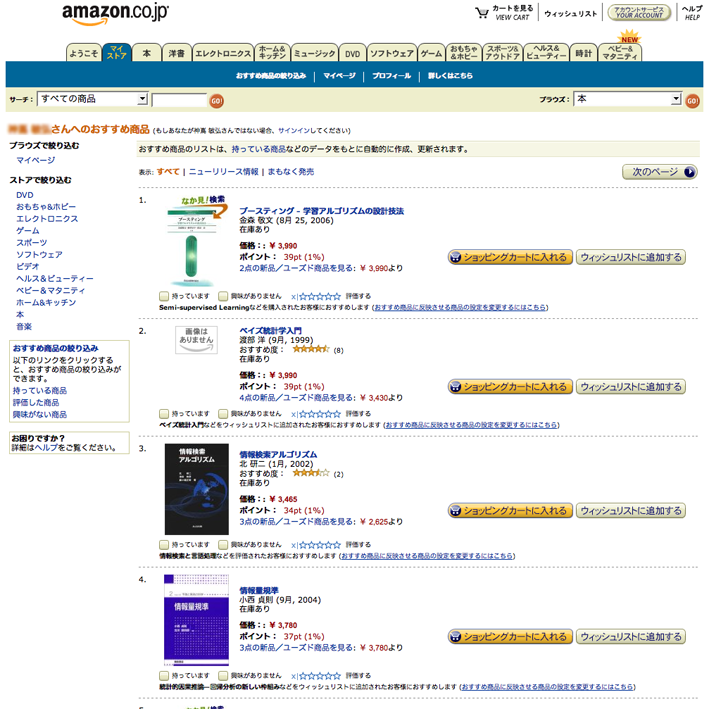
\includegraphics[width=0.48\linewidth]{pstyle1.png}}%
\hspace{0.02\linewidth}%
\subcaptionbox{評価値予測 (MovieLens~\cite{url:008})\label{fig:presentation:b}}%
{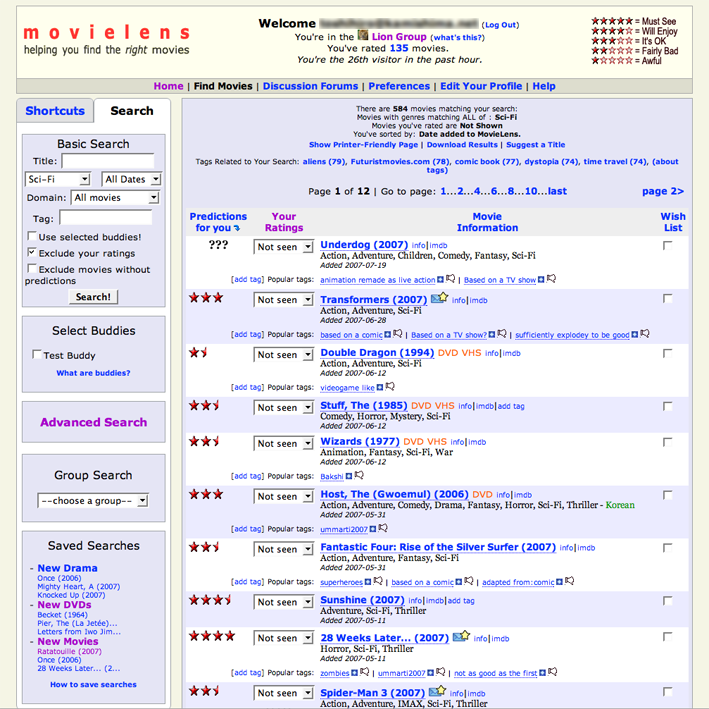
\includegraphics[width=0.48\linewidth]{pstyle2.png}}\\
\caption{推薦結果の表示例}
\label{fig:presentation}
{\footnotesize スクリーンショットは 2007/07/26 に取得した.}
\end{figure}

適合するものを一つ見つけ出す適合アイテム発見を目的とする場合には,予測される評価の高いものから順に整列したリストを利用者に提示するのが一般的である(図\ref{fig:presentation:a}).
%このリストの上位のアイテムほど,利用者の嗜好に適合する確率が高いだろう.
利用者はこのリストを上位から閲覧することで,自分の嗜好に適合したアイテムを素早く見つけることができる.

評価値予測で閲覧中にアイテムの評価を得ることを目的とする利用者は,積極的な決定をする意図をもっていない.
そこで,閲覧中のアイテムに,活動利用者の予測評価値を付随的に提示する.これは,★の数や,アイコン,グラフなどで表す(図\ref{fig:presentation:b}).
このような情報を参照することで,多数の候補の中から,利用者にとって関心のあるものを中心に閲覧できるようになる.

%利用者が自分の嗜好に適合するものを網羅的に見つけ出すことが目的である,適合アイテム列挙では,全ての候補を必ず利用者に提示しなくてはならない.

\section{多様性の向上}
\label{sec:serendipity}
\index{多様性}\index{diversity}
%@@@ 多様性の章に移行

評価値予測(\ref{sec:recomtask}節)を目的とする場合は,利用者の関心の幅を広げるため,多様性(\ref{sec:recomtype}節)の高い推薦が望まれる.
そこで,文献\cite{www:05:01}では多様性を向上させる目的で,予測精度を犠牲にしても,より広範囲の分野のアイテムを推薦する\term{話題多様化}{topic diversification}を提案している.
この多様化の有効性を,同種のアイテムに対しては,1度目より2度目,2度目より3度目に支払いたいと思う対価が減少する経済学における収穫逓減の法則 (law of diminishing marginal returns)との関連付けて論じている.
具体的には,アイテムの階層的な分類を導入し,分類階層の近さによってアイテム間の類似度を測る.
純粋に予測精度を重視したリストの上位から順に,最終推薦リストにアイテムを一つずつ追加するが,このとき,すでに推薦したアイテムと類似しているアイテムは推薦されにくいようにする.
この方法により,予測精度を犠牲にして,アイテムの多様性をより重視するような推薦をする実験を行った.
予測精度を単調に減少させ,徐々に多様性を高めると,最初は利用者は推薦の多様性の高まりを認知できたが,ある程度以上になると認知できなくなった.
よって,推薦リストの多様性を利用者が認知できる程度にとどめれば,予測精度もそれほど低下せず,利用者の満足は高まると報告している.
その他,推薦リストに,新製品やあまり知られていないアイテムを必ず混ぜるといった手法も考えられる\cite{sigir:01:01}.

\section{推薦理由}
\label{sec:explanation}
%@@@ 独立した章に

利用者は,不必要に高価なものを薦められていると疑ったりするため,推薦したアイテムを必ずしも採用するわけではない.
採用されない推薦は無意味なので,推薦ができるだけ採用されるような工夫が必要である.
そうした工夫として,アイテムの\term{推薦理由}{explanation of recommendations}も示すことが有効とされている.

文献\cite{sigchi:02:01}では,推薦の\term{透明性}{transparency}と利用者の推薦結果に与える印象との関係を調査している.
ここでいう透明性とは,利用者の入力した評価やその他の情報と,出力された推薦との間の因果関係が明確に説明されていることである.
この調査では,12人の被験者に5種類の商用音楽推薦システムを利用させた.
そして,推薦されたアイテムを好むか,推薦は信頼できるか,そして推薦に透明性があったかの質問をした.
調査の結果は,透明性があると考えた場合の方が,そうでない場合に比べて,有意に推薦された結果を好み,また,その結果を信頼できると答えた.
さらに,推薦されたアイテムを,(a)知らない場合,(b)知っていてかつそれを好きな場合,および(c)知っていてかつそれを嫌いな場合に分け
た.
推薦されたアイテムを好むかどうかの質問については,(b) (a) (c)の順に好んだ.
さらに,(a)と(b)の推薦については,推薦に透明性があると,ないときよりも,有意に推薦されたアイテムを好んだ.
しかし,(c)の推薦については,有意な差はなかった.
これらのことから,利用者が推薦に透明性があると考えたときには,推薦されたものをより好み,その推薦を信頼する.
また,知っている好きなアイテムを推薦されると,推薦に透明性があると利用者は考えるといえる.
なお,実際がどうであるかにかかわらず,透明性があると考えたかを利用者に質問した結果であること,また,システムがデータをねつ造していない点については,利用者はシステムを信頼していることには注意されたい.
利用者もおそらく知っているであろう,一般に知られたアイテムを推薦して,利用者の推薦への信頼を向上させるといったこともできる\cite{sigir:01:01}.

\begin{figure}
\centering
\subcaptionbox{類似した嗜好の利用者の評価の提示 \cite{cscw:00:01}\label{fig:explanation:a}}%
{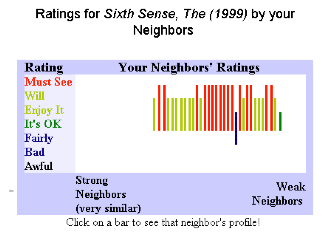
\includegraphics[width=0.48\linewidth]{Herlocker.png}}%
\hspace{0.02\linewidth}%
\subcaptionbox{推薦の根拠となった嗜好データの提示 (Amazon.co.jp)\label{fig:explanation:b}}%
{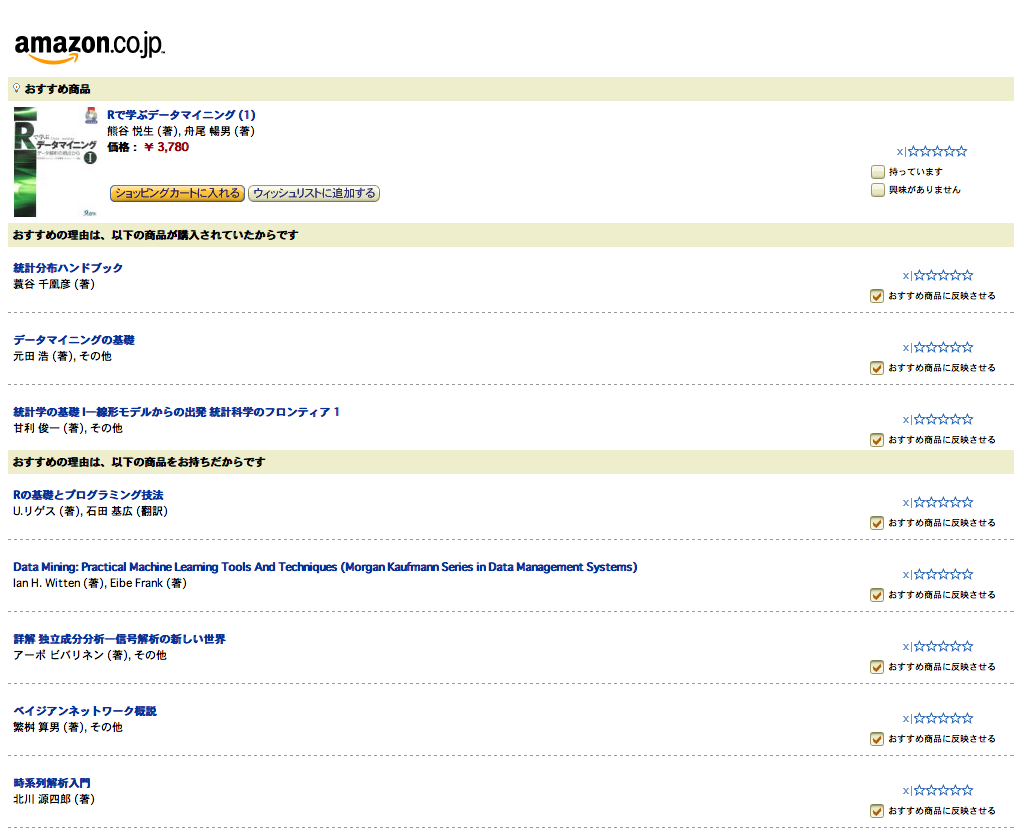
\includegraphics[width=0.48\linewidth]{explanation2.png}}\\
\caption{推薦理由の提示例}
\label{fig:explanation}
{\footnotesize スクリーンショットは 2007/07/26 に取得した.}
\end{figure}

推薦の透明性を高める,すなわち,利用者が入力した嗜好データから,推薦を導いた根拠を明示することで,推薦への信頼を高める試みがある.
文献\cite{cscw:00:01}では,こうした根拠を提示する手法を比較している.
その中で最も有効な方法とされたのが図\ref{fig:explanation:a}の方法である.
これは,活動利用者と類似した嗜好をもつ他の利用者の,推薦した映画についての評価値を棒グラフで示したものである.
この例では,推薦した映画について,嗜好が似ている人たちのほとんどが,最高か,それに次ぐ評価をしていることが,一目で分かる.
このように,推薦の手順の内部を示すアプローチを\term{ホワイトボックス}{whitebox}アプローチと呼ぶ.
その次に有効であったのは,そうした手順を示さない\term{ブラックボックス}{blackbox}アプローチの,推薦の確信度を示すことであった.
ここで,推薦の\term{強度}{strength}と\term{確信度}{confidence}について述べておこう.
推薦の強度とは,どれくらいアイテムを好むと予測しているかということである.
利用者の嗜好を5段階で予測するなら,5と予測したときに強い推薦といえる.
一方の推薦の確信度とは,この推薦をどれくらい確かだと考えているかということである.
\ref{sec:probmodel}節の確率モデルで,適合/不適合の2段階で活動利用者の嗜好を予測したとしよう.
このとき,適合すると予測した確率が$0.6$でも$0.9$でも,予測は「適合」だが,後者のときにより確かな推薦といえる.
さらに,他の方法でも実験したが,利用者の満足を向上させた方法は無かったと報告している.

その他,\ref{sec:item-item}節のようにアイテム間の類似度に基づく推薦では,推薦に関連したアイテムを提示するというホワイトボックスアプローチもある.
図\ref{fig:explanation:b}は,活動利用者自身の,推薦の根拠となった他のアイテムへの評価を提示したものである.
また,暗黙的に嗜好データを獲得した場合,推薦の根拠を利用者が認知できなくなるので,推薦と共に根拠となった嗜好データを示す方法もある.
ただし,予測評価値などを提示して,利用者が嫌いなアイテムが高評価されていると,システムに対する信頼を失う危険性も指摘されている\cite{sigir:01:01}.


%!TEX root =  main.tex
%!TEX encoding = UTF-8 Unicode





% privacy
\nocite{kdd:09:01} % 差分プライバシのCF
\nocite{misc:003} % 差分プライバシの基本文献

% social recommendation
\nocite{ec:041}

% popularity bias, diversity
\nocite{misc:011} % PRPの基本文献
\nocite{ej:055}
\nocite{kdd:08:04}
\nocite{recsys:10:01}
\nocite{sigchi:08:01} % bandwagon effect
\nocite{url:005} % LongTailの基本文献

% evaluation
\nocite{etr:008} % ABテストで利用者に悪い影響が残る

% memory-based
\nocite{icdm:07:01} % 近隣法のバイアスとか

% web content optimization
\nocite{jml:02:03} % UCB1
\nocite{icdm:09:01}
\nocite{icml:99:02}
\nocite{www:10:01}

% RBM
\nocite{icml:07:05}

% matrix factorization
\nocite{kdd:08:05}
\nocite{kdd:09:02} % 時間付き
\nocite{kdd:09:03} % テンソル分解,タグ推薦
\nocite{misc:012} % 欠損の考慮
\nocite{url:009} % 確率的勾配降下

% preference elicitation
\nocite{recsys:11:01}


% ===== Back Matter =====
\backmatter
\singlespacing

% ---- Acknowledgements ----
%\medskip
%\noindent\small\textbf{謝辞}:\ 
%みんなありがとう

% ---- Bibliography ----
\bibliographystyle{jsai}
\bibliography{ebib,epublist,emisc,jbib,jpublist,jmisc}

% --- Indexes ---
\printindex

\end{document}
